\documentclass{article}
\usepackage{graphicx} % Required for inserting images

% remove equation auto numbering
\usepackage{amsmath}

% for the image grid
\usepackage{subcaption}

% arrows
\usepackage{tikz}
\usetikzlibrary{arrows.meta}

% links
\usepackage{hyperref}
\hypersetup{
    colorlinks=true,
    linkcolor=blue,
    filecolor=magenta,      
    urlcolor=blue
    }

% make enumeration start from 0
\usepackage{enumitem}

% highlighted code
\usepackage{minted}

% block comments
\usepackage{comment}

\title{\textbf{Vision \& Perception}}
\author{Daniel Gigliotti}
\date{}

% section dots in toc
\usepackage{etoolbox}
\makeatletter
\patchcmd{\l@section}
  {\hfil}
  {\leaders\hbox{\normalfont$\m@th\mkern \@dotsep mu\hbox{.}\mkern \@dotsep mu$}\hfill}
  {}{}
\makeatother

% non-maximum suppression image
\def\pixelmap{{%
{2,2,2,1,0,0,0,0,0},
{1,2,2,1,0,0,1,0,0},
{1,1,2,2,2,1,0,0,0},
{0,1,1,2,2,1,1,0,0},
{0,1,1,1,2,2,1,1,0},
{0,0,0,1,2,2,2,1,0},
{0,0,0,0,1,2,2,2,1},
{0,0,0,0,1,1,2,2,1},
{0,0,0,1,0,1,2,2,2},
}}

\colorlet{color0}{white}
\colorlet{color1}{gray}
\colorlet{color2}{black}

\begin{document}

\maketitle

\tableofcontents

\newpage

\addcontentsline{toc}{section}{Images as functions}
\section*{Images as functions}

An image is a 3D tensor of numbers. 

We can think of an image as a function 

\begin{equation*}
f:R^2 \rightarrow R
\end{equation*}

\begin{equation*}
    \begin{split}
    f: [a\ & \times \ b][c\ \times\ d] \rightarrow [0,\ 255] \\
    & domain\ \ \ \ \ \ \ \ \ \ \ \ \ range
    \end{split}
\end{equation*}

$f(x, y)$ gives the intensity at position (x, y). A digital image is a discrete (sampled, quantized) version of this function:

\begin{itemize}
    \item \textbf{sampling} $\rightarrow$ sample a 2D space on a grid
    \item \textbf{quantization} $\rightarrow$ clip the value in a grid cell to a specific range (0, 255)
\end{itemize}

\begin{equation*}
    f(i, j) = quantize(i\Delta, j\Delta)
\end{equation*}

This formulation holds for single-channel images. A color image is composed of three channels and can be seen as three functions pasted together.

\begin{equation*}
    f(x,y)= \begin{bmatrix}
        r(x,y) \\
       g(x,y) \\
       b(x,y)
    \end{bmatrix}
\end{equation*}

\newpage

\begin{center}
    \begin{tabular}{llll}
        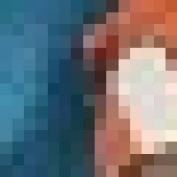
\includegraphics[width=.2\linewidth]{images/color.png} \hspace{2cm} & 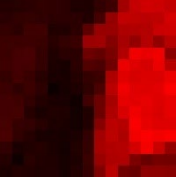
\includegraphics[width=.2\linewidth]{images/r.png} &   
        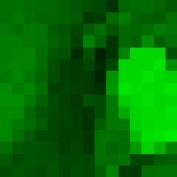
\includegraphics[width=.2\linewidth]{images/g.png} &
        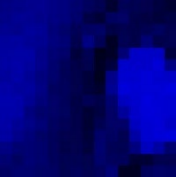
\includegraphics[width=.2\linewidth]{images/b.png} \\
        \hspace{0.2cm} \\
        \text{color image patch} & 
        \text{R channel} &
        \text{G channel} &
        \text{B channel} \\
        \hspace{1cm} \\
        \text{actual intensity per channel:} & 
        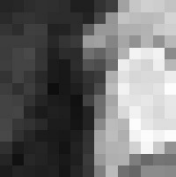
\includegraphics[width=.2\linewidth]{images/r_.png} &   
        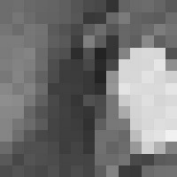
\includegraphics[width=.2\linewidth]{images/g_.png} &
        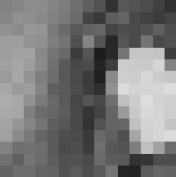
\includegraphics[width=.2\linewidth]{images/b_.png} \\
    \end{tabular}
\end{center}

\newpage

\addcontentsline{toc}{section}{Image processing}
\section*{Image processing}

We have two types of image processing:

\begin{itemize}
    \item \textbf{image warping} changes the domain (pixel positions) of the image; points
are mapped to other points without changing their colors;
    \item \textbf{image filtering} changes the range (pixel values) of the image; the colors of the image are altered without changing the individual pixel position; 
\end{itemize}

\addcontentsline{toc}{section}{Image filtering}
\section*{Image filtering}

We have two types of image filtering:

\begin{itemize}
    \item \textbf{point processing}: change the range of a pixel only accounting for its current value;
    \item \textbf{neighborhood processing}: change the range of a pixel taking into account the values of its neighbors;
\end{itemize}

Filtering allows us to make a new image whose pixels are a combination of the original pixels in the corresponding area. We modify the pixels in an image based on some function of a local neighborhood, in the source image, of each pixel. Filters can be both linear and non-linear.

\begin{center}
    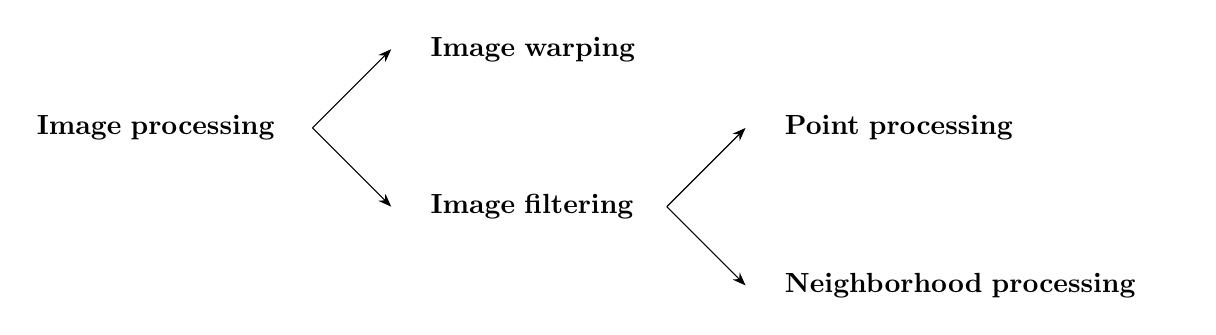
\begin{tikzpicture}
        \node[text width = 5cm] at (0, 0) {\textbf{Image processing}};
        \draw[-{Stealth[black]}] (1,0) -- (2,1);
        \draw[-{Stealth[black]}] (1,0) -- (2,-1);
        \node[text width = 5cm] at (5, 1) {\textbf{Image warping}};
        \node[text width = 5cm] at (5, -1) {\textbf{Image filtering}};
        \draw[-{Stealth[black]}] (5.5,-1) -- (6.5,0);
        \draw[-{Stealth[black]}] (5.5,-1) -- (6.5,-2);
        \node[text width = 5cm] at (9.5, 0) {\textbf{Point processing}};
        \node[text width = 5cm] at (9.5, -2) {\textbf{Neighborhood processing}};
    \end{tikzpicture}
\end{center}

\newpage

\addcontentsline{toc}{section}{Point processing}
\section*{Point processing}

Point processing in image filtering is a technique where a single pixel in an image is processed independently of its neighboring pixels. This is in contrast to neighborhood (or spatial) processing, where the value of a pixel is determined by the values of neighboring ones.

Examples of point processing include:
\begin{itemize}
    \item \textbf{brightness and contrast adjustment}: this involves adjusting the overall brightness and contrast of an image by multiplying the value of each pixel by a constant factor;
    \item \textbf{gamma correction}: this involves adjusting the brightness of an image by applying a non-linear transformation to pixel values;
    \item \textbf{histogram equalization}: this involves adjusting the distribution of pixel values in an image to improve its overall contrast;
    \item \textbf{thresholding}: this involves converting every pixel within a certain range to have a fixed value;
    \item \textbf{color balance}: this involves adjusting the color balance of an image by altering the relative intensities of its color channels;
    \item \textbf{colorization}: this involves adding color information to a gray-scale image by mapping the intensity values to a color map;
    \item \textbf{negation}: this involves inverting the color of an image by subtracting the pixel values from the maximum value (255);
\end{itemize}

\newpage

\addcontentsline{toc}{section}{Convolution and correlation}
\section*{Convolution and correlation}

Correlation and convolution are both mathematical operations that are used in signal processing and image processing. 

They involve multiplying a signal/image by a filter kernel. The result of this operation is a new image where each pixel is a weighted sum of the pixels in the original image, but there are important differences between the two.

\addcontentsline{toc}{section}{Correlation}
\section*{Correlation}

Definition for 2D correlation for image filtering:

\begin{equation*}
    (f \otimes g)(x, y) = \sum_{i = -k}^{k} \sum_{j = -k}^{k} f(i, j)I(x+i, y+j)
\end{equation*}

\begin{center}
    \textit{$f(i, j)$ is the kernel} \\
    \textit{$I(x+i, j+j)$ is the input image} \\
    \textit{$(f \otimes g)(x, y)$ is the filtered image}
\end{center}

Notice the lack of a flip in $I(x+i, y+j)$.

\addcontentsline{toc}{section}{Convolution}
\section*{Convolution}

Definition for 2D convolution for image filtering:

\begin{equation*}
    (f * g)(x, y) = \sum_{i=-k}^{k} \sum_{j=-k}^{k} f(i, j)I(x-i, y-j)    
\end{equation*}

\begin{center}
    \textit{$f(i, j)$ is the kernel} \\
    \textit{$I(x-i, j-j)$ is the input image} \\
    \textit{$(f*g)(x, y)$ is the filtered image}
\end{center}

The patch is flipped both horizontally and vertically.

\addcontentsline{toc}{section}{Correlation and Convolution order}
\section*{Correlation and Convolution order}

Right: correlation order in the linear combination \\ 
Left: convolution order in the linear combination

\vspace{0.1cm}

\begin{center}
    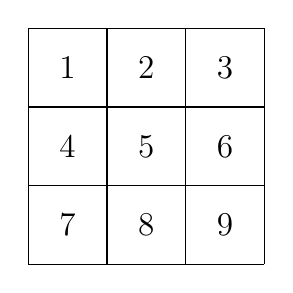
\begin{tikzpicture}
        \draw[step=1cm,color=black] (0, 0) grid (3,3);
        \node[font = {\large}, black] at (0.5, 2.5) {1};
        \node[font = {\large}, black] at (1.5, 2.5) {2};
        \node[font = {\large}, black] at (2.5, 2.5) {3};
        \node[font = {\large}, black] at (0.5, 1.5) {4};
        \node[font = {\large}, black] at (1.5, 1.5) {5};
        \node[font = {\large}, black] at (2.5, 1.5) {6};
        \node[font = {\large}, black] at (0.5, 0.5) {7};
        \node[font = {\large}, black] at (1.5, 0.5) {8};
        \node[font = {\large}, black] at (2.5, 0.5) {9};
    \end{tikzpicture}
    \ \ \ \ \ \ \ \ \ \ \ \ \ \ 
    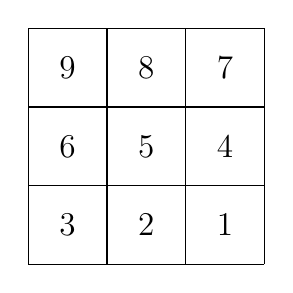
\begin{tikzpicture}
        \draw[step=1cm,color=black] (0, 0) grid (3,3);
        \node[font = {\large}, black] at (0.5, 2.5) {9};
        \node[font = {\large}, black] at (1.5, 2.5) {8};
        \node[font = {\large}, black] at (2.5, 2.5) {7};
        \node[font = {\large}, black] at (0.5, 1.5) {6};
        \node[font = {\large}, black] at (1.5, 1.5) {5};
        \node[font = {\large}, black] at (2.5, 1.5) {4};
        \node[font = {\large}, black] at (0.5, 0.5) {3};
        \node[font = {\large}, black] at (1.5, 0.5) {2};
        \node[font = {\large}, black] at (2.5, 0.5) {1};
    \end{tikzpicture}
\end{center}

\newpage

\addcontentsline{toc}{section}{Padding}
\section*{Padding}

Just applying the convolution operator will reduce the size of the image and this is not always desirable. \textbf{Padding} refers to the technique of adding extra rows and columns of zeros around the edges of the image. Padding is commonly used to preserve spatial dimensions during convolutional operations and to prevent information loss at the edges of the feature map.

There are three common types of padding:

\begin{itemize}
    \item \textbf{Same padding}: the input image is padded with zeros in such a way that the output has the same spatial dimensions as the input. This is achieved by adding $\lfloor((filter\_size - 1) / 2)\rfloor$ rows and columns of zeros on both sides.
    \item \textbf{Valid padding}: the input image is not padded at all. This means that the filter is only applied to positions where it can completely overlap with the input. As a result, the output has smaller spatial dimensions.    
    \item \textbf{Full padding}: the input is padded with zeros in such a way that the output has the maximum possible spatial dimensions. This is achieved by adding $\lfloor(filter\_size - 1)\rfloor$ rows and columns of zeros on both sides. The resulting output has larger spatial dimensions.
\end{itemize}

\newpage

\addcontentsline{toc}{section}{Filters}
\section*{Filters}

The operations applied with \textbf{filters} are typically convolutions and correlations. In both cases we replace a pixel in the new image with a combination (a weighted sum) of the respective pixel in the old image and its neighbors. The neighbors are multiplied by a set of coefficients, known as \textbf{kernel}. \\

\vspace{0.5cm}

Convolution between an image patch and the box filter:
\begin{center}
    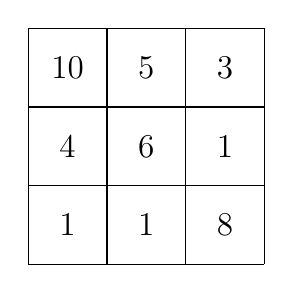
\begin{tikzpicture}
        \draw[step=1cm,color=black] (0, 0) grid (3,3);
        \node[font = {\large}, black] at (0.5, 0.5) {1};
        \node[font = {\large}, black] at (1.5, 0.5) {1};
        \node[font = {\large}, black] at (2.5, 0.5) {8};
        \node[font = {\large}, black] at (0.5, 1.5) {4};
        \node[font = {\large}, black] at (1.5, 1.5) {6};
        \node[font = {\large}, black] at (2.5, 1.5) {1};
        \node[font = {\large}, black] at (0.5, 2.5) {10};
        \node[font = {\large}, black] at (1.5, 2.5) {5};
        \node[font = {\large}, black] at (2.5, 2.5) {3};
    \end{tikzpicture}
    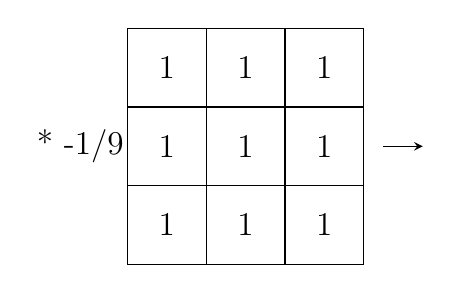
\begin{tikzpicture}
        \draw[step=1cm,color=black] (0, 0) grid (3,3);
        \node[font = {\large}, black] at (0.5, 0.5) {1};
        \node[font = {\large}, black] at (1.5, 0.5) {1};
        \node[font = {\large}, black] at (2.5, 0.5) {1};
        \node[font = {\large}, black] at (0.5, 1.5) {1};
        \node[font = {\large}, black] at (1.5, 1.5) {1};
        \node[font = {\large}, black] at (2.5, 1.5) {1};
        \node[font = {\large}, black] at (0.5, 2.5) {1};
        \node[font = {\large}, black] at (1.5, 2.5) {1};
        \node[font = {\large}, black] at (2.5, 2.5) {1};
        
        \node[font = {\large}, black] at (-0.6, 1.5) {*\ -1/9};

        \draw [-stealth](3.25,1.5) -- (3.75,1.5);
    \end{tikzpicture}
    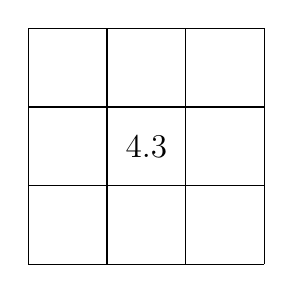
\begin{tikzpicture}
        \draw[step=1cm,color=black] (0, 0) grid (3,3);
        \node[font = {\large}, black] at (0.5, 0.5) {};
        \node[font = {\large}, black] at (1.5, 0.5) {};
        \node[font = {\large}, black] at (2.5, 0.5) {};
        \node[font = {\large}, black] at (0.5, 1.5) {};
        \node[font = {\large}, black] at (1.5, 1.5) {4.3};
        \node[font = {\large}, black] at (2.5, 1.5) {};
        \node[font = {\large}, black] at (0.5, 2.5) {};
        \node[font = {\large}, black] at (1.5, 2.5) {};
        \node[font = {\large}, black] at (2.5, 2.5) {};
    \end{tikzpicture}
\end{center}

Convolution between an image patch and a custom filter:
\begin{center}
    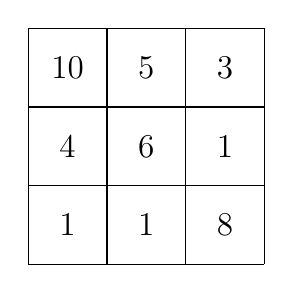
\begin{tikzpicture}
        \draw[step=1cm,color=black] (0, 0) grid (3,3);
        \node[font = {\large}, black] at (0.5, 0.5) {1};
        \node[font = {\large}, black] at (1.5, 0.5) {1};
        \node[font = {\large}, black] at (2.5, 0.5) {8};
        \node[font = {\large}, black] at (0.5, 1.5) {4};
        \node[font = {\large}, black] at (1.5, 1.5) {6};
        \node[font = {\large}, black] at (2.5, 1.5) {1};
        \node[font = {\large}, black] at (0.5, 2.5) {10};
        \node[font = {\large}, black] at (1.5, 2.5) {5};
        \node[font = {\large}, black] at (2.5, 2.5) {3};
    \end{tikzpicture}
    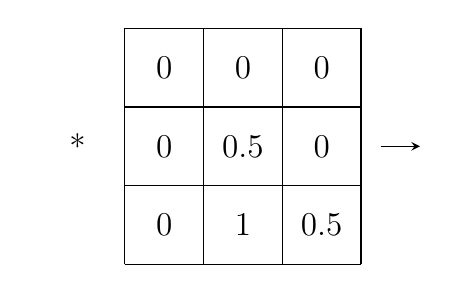
\begin{tikzpicture}
        \draw[step=1cm,color=black] (0, 0) grid (3,3);
        \node[font = {\large}, black] at (0.5, 0.5) {0};
        \node[font = {\large}, black] at (1.5, 0.5) {1};
        \node[font = {\large}, black] at (2.5, 0.5) {0.5};
        \node[font = {\large}, black] at (0.5, 1.5) {0};
        \node[font = {\large}, black] at (1.5, 1.5) {0.5};
        \node[font = {\large}, black] at (2.5, 1.5) {0};
        \node[font = {\large}, black] at (0.5, 2.5) {0};
        \node[font = {\large}, black] at (1.5, 2.5) {0};
        \node[font = {\large}, black] at (2.5, 2.5) {0};

        \node[font = {\large}, black] at (-0.6, 1.5) {\ \ \ *\ \ \ \ };
        
        \draw [-stealth](3.25,1.5) -- (3.75,1.5);
    \end{tikzpicture}
    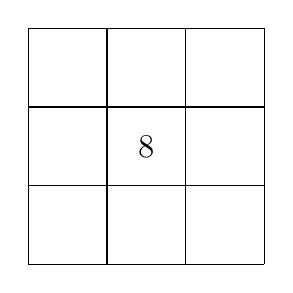
\begin{tikzpicture}
        \draw[step=1cm,color=black] (0, 0) grid (3,3);
        \node[font = {\large}, black] at (0.5, 0.5) {};
        \node[font = {\large}, black] at (1.5, 0.5) {};
        \node[font = {\large}, black] at (2.5, 0.5) {};
        \node[font = {\large}, black] at (0.5, 1.5) {};
        \node[font = {\large}, black] at (1.5, 1.5) {8};
        \node[font = {\large}, black] at (2.5, 1.5) {};
        \node[font = {\large}, black] at (0.5, 2.5) {};
        \node[font = {\large}, black] at (1.5, 2.5) {};
        \node[font = {\large}, black] at (2.5, 2.5) {};
    \end{tikzpicture}
\end{center}

\vspace{0.5cm}

If the kernel is constant while shifting it on all the pixel locations, the filter is called \textbf{shift invariant} (all the pixels use the same linear combination of their neighbors). \\

\textbf{Linear filters} can be implemented quickly and efficiently, but they can also be less effective than \textbf{non-linear filters} for certain types of image processing tasks. However, they are widely used due to their simplicity and effectiveness.

\newpage

A 2D filter is \textbf{separable} if it can be written as the product of a column and a row vector:

\begin{center}
    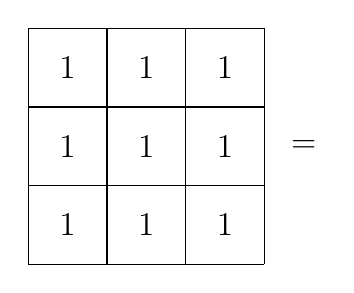
\begin{tikzpicture}
        \draw[step=1cm,color=black] (0, 0) grid (3,3);
        \node[font = {\large}, black] at (0.5, 0.5) {1};
        \node[font = {\large}, black] at (1.5, 0.5) {1};
        \node[font = {\large}, black] at (2.5, 0.5) {1};
        \node[font = {\large}, black] at (0.5, 1.5) {1};
        \node[font = {\large}, black] at (1.5, 1.5) {1};
        \node[font = {\large}, black] at (2.5, 1.5) {1};
        \node[font = {\large}, black] at (0.5, 2.5) {1};
        \node[font = {\large}, black] at (1.5, 2.5) {1};
        \node[font = {\large}, black] at (2.5, 2.5) {1};

        \node[font = {\large}, black] at (3.5, 1.5) {=};
    \end{tikzpicture}
    \begin{tikzpicture}
        \draw[step=1cm,color=black] (0, 0) grid (1,3);
        \node[font = {\large}, black] at (0.5, 0.5) {1};
        \node[font = {\large}, black] at (0.5, 1.5) {1};
        \node[font = {\large}, black] at (0.5, 2.5) {1};

        \node[font = {\large}, black] at (1.5, 1.5) {$\times$};

        \draw[step=1cm,color=black] (2, 2) grid (5,3);
        \node[font = {\large}, black] at (2.5, 2.5) {1};
        \node[font = {\large}, black] at (3.5, 2.5) {1};
        \node[font = {\large}, black] at (4.5, 2.5) {1};
    \end{tikzpicture}
\end{center}

2D convolution with a separable filter is equivalent to two 1D convolutions (with the column and row filters). If the image has $m \times n$ pixels and the kernel filter has size $l \times l$:

\begin{itemize}
    \item the cost of a convolution with a non-separable filter is $l^2 \times (m \times n)$
    \item the cost of a convolution with a separable filter is $2 \times (l \times (m \times n))$
\end{itemize}

It is always convenient to use separable filters.

\addcontentsline{toc}{section}{Box filter}
\section*{Box filter }

The box filter is the simplest kind of filter we can imagine: it simply takes the average of all the pixels under the kernel area. It is linear (it fulfills both the superposition and the homogeneity principles) and separable (can be written as a product of of a column and a row vector). 

The box filter takes the average of the pixels under the kernel area. By doing so, it smoothes out the image, reducing noise. It helps suppressing sharp transitions, however it also tends to blur edges and fine details along with the noise, which may not be desirable in certain applications.

\vspace{0.5cm}

Convolution between an image patch and the box filter:
\begin{center}
    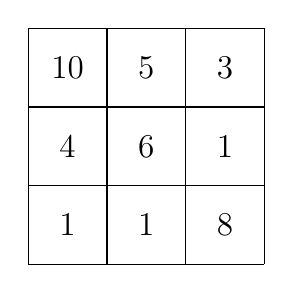
\begin{tikzpicture}
        \draw[step=1cm,color=black] (0, 0) grid (3,3);
        \node[font = {\large}, black] at (0.5, 0.5) {1};
        \node[font = {\large}, black] at (1.5, 0.5) {1};
        \node[font = {\large}, black] at (2.5, 0.5) {8};
        \node[font = {\large}, black] at (0.5, 1.5) {4};
        \node[font = {\large}, black] at (1.5, 1.5) {6};
        \node[font = {\large}, black] at (2.5, 1.5) {1};
        \node[font = {\large}, black] at (0.5, 2.5) {10};
        \node[font = {\large}, black] at (1.5, 2.5) {5};
        \node[font = {\large}, black] at (2.5, 2.5) {3};
    \end{tikzpicture}
    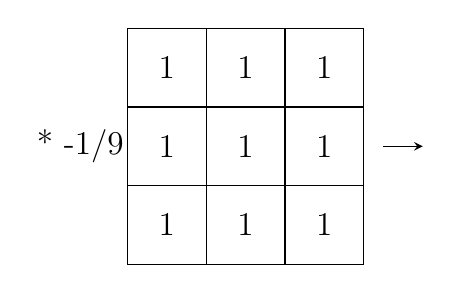
\begin{tikzpicture}
        \draw[step=1cm,color=black] (0, 0) grid (3,3);
        \node[font = {\large}, black] at (0.5, 0.5) {1};
        \node[font = {\large}, black] at (1.5, 0.5) {1};
        \node[font = {\large}, black] at (2.5, 0.5) {1};
        \node[font = {\large}, black] at (0.5, 1.5) {1};
        \node[font = {\large}, black] at (1.5, 1.5) {1};
        \node[font = {\large}, black] at (2.5, 1.5) {1};
        \node[font = {\large}, black] at (0.5, 2.5) {1};
        \node[font = {\large}, black] at (1.5, 2.5) {1};
        \node[font = {\large}, black] at (2.5, 2.5) {1};
        
        \node[font = {\large}, black] at (-0.6, 1.5) {*\ -1/9};

        \draw [-stealth](3.25,1.5) -- (3.75,1.5);
    \end{tikzpicture}
    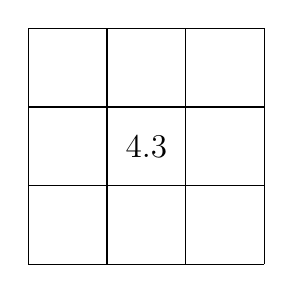
\begin{tikzpicture}
        \draw[step=1cm,color=black] (0, 0) grid (3,3);
        \node[font = {\large}, black] at (0.5, 0.5) {};
        \node[font = {\large}, black] at (1.5, 0.5) {};
        \node[font = {\large}, black] at (2.5, 0.5) {};
        \node[font = {\large}, black] at (0.5, 1.5) {};
        \node[font = {\large}, black] at (1.5, 1.5) {4.3};
        \node[font = {\large}, black] at (2.5, 1.5) {};
        \node[font = {\large}, black] at (0.5, 2.5) {};
        \node[font = {\large}, black] at (1.5, 2.5) {};
        \node[font = {\large}, black] at (2.5, 2.5) {};
    \end{tikzpicture}
\end{center}

\newpage

\addcontentsline{toc}{section}{Gaussian filter}
\section*{Gaussian filter}

\textbf{Gaussian filter} uses the Gaussian function to smooth images and reduce noise; The Gaussian function is a bell-shaped curve that gives more weight to pixels in the center of the filter and less weight to pixels at the edges (weight falls off with distance from center); the resulting smoothing effect preserves edges and details in the image better than box filter; a Gaussian effect can be obtained from a convolution between the image and a Gaussian function; \\

\hspace{0.5cm}

\begin{center}
    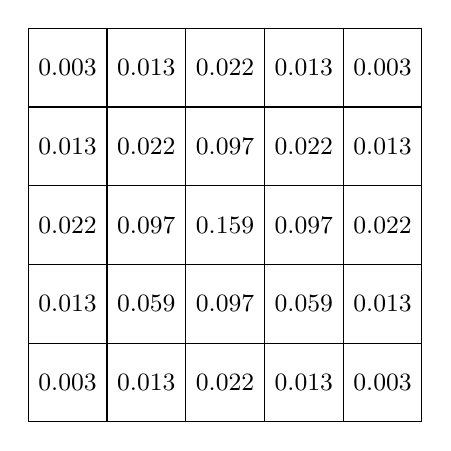
\begin{tikzpicture}
        \draw[step=1cm,color=black] (0, 0) grid (5,5);

        % first row
        \node[font = {\small}, black] at (0.5, 0.5) {0.003};
        \node[font = {\small}, black] at (1.5, 0.5) {0.013};
        \node[font = {\small}, black] at (2.5, 0.5) {0.022};
        \node[font = {\small}, black] at (3.5, 0.5) {0.013};
        \node[font = {\small}, black] at (4.5, 0.5) {0.003};
        
        % second row
        \node[font = {\small}, black] at (0.5, 1.5) {0.013};
        \node[font = {\small}, black] at (1.5, 1.5) {0.059};
        \node[font = {\small}, black] at (2.5, 1.5) {0.097};
        \node[font = {\small}, black] at (3.5, 1.5) {0.059};
        \node[font = {\small}, black] at (4.5, 1.5) {0.013};

        % third row
        \node[font = {\small}, black] at (0.5, 2.5) {0.022};
        \node[font = {\small}, black] at (1.5, 2.5) {0.097};
        \node[font = {\small}, black] at (2.5, 2.5) {0.159};
        \node[font = {\small}, black] at (3.5, 2.5) {0.097};
        \node[font = {\small}, black] at (4.5, 2.5) {0.022};

        % fourth row
        \node[font = {\small}, black] at (0.5, 3.5) {0.013};
        \node[font = {\small}, black] at (1.5, 3.5) {0.022};
        \node[font = {\small}, black] at (2.5, 3.5) {0.097};
        \node[font = {\small}, black] at (3.5, 3.5) {0.022};
        \node[font = {\small}, black] at (4.5, 3.5) {0.013};

        % fifth row
        \node[font = {\small}, black] at (0.5, 4.5) {0.003};
        \node[font = {\small}, black] at (1.5, 4.5) {0.013};
        \node[font = {\small}, black] at (2.5, 4.5) {0.022};
        \node[font = {\small}, black] at (3.5, 4.5) {0.013};
        \node[font = {\small}, black] at (4.5, 4.5) {0.003};

    \end{tikzpicture}
\end{center}
Above, weight contributions of neighboring pixels by nearness in a $5x5$ Gaussian filter with $\sigma = 1$. The kernel values are sampled from the 2D Gaussian function:

\begingroup
\Large
\begin{equation*}
    f(i,j) = \frac{1}{2 \pi \sigma^2} e^{-\frac{i^2+j^2}{2 \sigma^2}}
\end{equation*}
\endgroup

Weights fall off with distance from the center pixel. The kernel can theoretically be infinite but in practice it is truncated to some maximum distance. Selecting where to truncate the distance of a Gaussian filter depends on the specific application and the desired level of smoothing. However, a common heuristic for selecting the truncation distance is to choose the distance at which the Gaussian function falls to a certain percentage of its maximum value. \\

For example, one common choice is to truncate the Gaussian filter at a distance where the Gaussian function falls to 1\% or less of its maximum value. This means that the filter will consider only the pixels within a certain radius from the center of the filter, and pixels farther away will not have a significant effect on the output image. \\

Another heuristic for selecting the truncation distance is to use the standard deviation of the Gaussian distribution. The standard deviation determines the width of the Gaussian function, and choosing the truncation distance based on the standard deviation ensures that the filter considers only the most relevant pixels within a certain distance from the center of the filter.

\addcontentsline{toc}{section}{Difference between Gaussian filter and Box filter}
\section*{Difference between Gaussian filter and Box filter}

Gaussian filter and box filter are two commonly used image smoothing filters in image processing. Although \textbf{both filters are used for the same purpose of reducing noise and smoothing an image}, they produce different results due to their different characteristics. \\

The main difference between a Gaussian filter and a box filter is that a Gaussian filter uses a Gaussian function to calculate the weights of the neighboring pixels, while a box filter uses a uniform weight for all neighboring pixels within a given window. \\

In terms of the output image, the main difference between the two filters is the level of smoothing and blurring that they produce. \textbf{A Gaussian filter produces a smoother output image with less blurring compared to a box filter}. This is because the Gaussian filter assigns higher weights to the pixels closer to the center of the filter window and lower weights to the pixels farther away, resulting in a smoother transition between neighboring pixels. In contrast, \textbf{a box filter assigns equal weights to all neighboring pixels, resulting in a more uniform smoothing and potential blurring of edges and details in the image}. \\

Therefore, if the goal is to reduce noise and smooth the image while preserving the edges and details, a Gaussian filter is generally preferred. On the other hand, if the goal is to simply reduce noise and blur the image uniformly, a box filter may be more suitable. However, it is important to note that the choice of filter depends on the specific application and the desired level of smoothing, and it may require some experimentation to find the most appropriate filter for a given image processing task. \\

In the frequency domain, the box filter and the Gaussian filter have different effects on the image:

\begin{itemize}
    \item the \textbf{box filter} has a rectangular frequency response, which \textbf{leads to a sinc-like function in the spatial domain}. The sinc function has oscillations, which can lead to \textbf{ringing} artifacts in the image (ripple like structures);
    \item the \textbf{Gaussian filter} has a smooth, bell-shaped frequency response. This results in a smoother, more gradual transition between the filtered and unfiltered regions of the image. Gaussian filtering typically \textbf{produces fewer ringing artifacts} than box filtering;
\end{itemize}

\newpage

\addcontentsline{toc}{section}{Sharpening filters}
\section*{Sharpening filters}

A sharpening filter is a type of image filter that enhances the edges and details of an image, making it appear sharper. It works by amplifying the high-frequency components of the image, which correspond to the edges and fine details (edges and fine details are high frequency components because there is rapid change in pixel intensity or color). \\

To obtain a sharpening filter from an original image and a blurring filter, we can use a technique called \textbf{unsharp masking}. 
Here are the steps:

\begin{itemize}
    \item Apply the blurring filter to the original image (low frequency components).
    \item Subtract the blurred image from the original image to obtain the high-frequency components.
    \item Add the result back to the original image. This will create a sharpened version of the image.
\end{itemize}

The resulting filter can be applied to other images to enhance their sharpness. However, it's important to note that this technique can also amplify noise in the image, so it should be used with caution.

\addcontentsline{toc}{section}{Linear and non-linear filter}
\section*{Linear and non-linear filters}

\begin{table}[h!]
\centering
\begin{tabular}{c|c}

\textbf{Linear Filters} & \textbf{Non-Linear Filters} \\
Gaussian Filter & Median Filter \\
Mean Filter & Bilateral Filter \\
Box Filter & Non-local Means Filter \\
Sobel Filter & Maximum Filter \\
Laplacian Filter & Minimum Filter \\
\end{tabular}
\caption{Examples of Linear and Non-Linear Image Filters}
\label{tab:filters}
\end{table}

\newpage

\addcontentsline{toc}{section}{Why is the Gaussian filter linear?}
\section*{Why is the Gaussian filter linear?}

The Gaussian filter is a linear filter because it satisfies the two fundamental properties of linearity: \textbf{superposition} and \textbf{homogeneity}.\

\begin{itemize}
    \item \textbf{Superposition} means that the response of the filter to a sum of inputs is equal to the sum of the responses to each input. In other words, if we apply the filter to a weighted sum of two images, the resulting output will be the weighted sum of the filtered versions of each image. The Gaussian filter satisfies this property because it convolves the input image with a linear, separable kernel that can be expressed as the sum of two 1D Gaussian functions.
    \item \textbf{Homogeneity} means that the response of the filter is proportional to the input signal. In other words, if we scale the input signal by a constant factor, the output of the filter will also be scaled by the same factor. The Gaussian filter satisfies this property because it convolves the input image with a kernel that is a function of the distance from the center of the kernel, and this distance is proportional to the magnitude of the input signal.
\end{itemize}

In layman's terms, a filter is linear if its response to a sum of two signals is the same as the sum of the individual responses. This is equivalent to saying that each output pixel is a weighted summation of some number of input pixels. This is not true for non-linear filters, like the Maximum filter, where the output pixel is the maximum among the pixels in the considered window. 

\addcontentsline{toc}{section}{Why is the Gaussian filter separable?}
\section*{Why is the Gaussian filter separable?}

The Gaussian filter is separable because it can be expressed as the convolution of two 1D Gaussian filters, one applied horizontally and one applied vertically (the proof is omitted). We can apply these filters separately to achieve the same result as applying the full 2D Gaussian filter, but with less computational cost. This is the key reason why the Gaussian filter is commonly used in image processing applications.

\newpage 

\addcontentsline{toc}{section}{Feature Detection and Feature Description}
\section*{Feature Detection and Feature Description}

\textbf{Feature detection} is the process of finding key points or regions in an image that are relevant for a specific task, such as object recognition or image matching. For example, feature detectors like SIFT (Scale-Invariant Feature Transform) or SURF (Speeded Up Robust Features) can identify distinctive points in an image, such as corners or edges, which can be used to describe the image. \\

Commonly used feature detection algorithms are:
\begin{itemize}
    \item Harris Corner Detector
    \item Canny Edge Detector
    \item Scale Invariant Feature Transform (SIFT) Detector
    \item Speeded-Up Robust Features (SURF) Detector
\end{itemize}

\textbf{Feature description}, on the other hand, is the process of representing the key points or regions identified by feature detection in a compact and meaningful way. The goal of feature description is to create a representation that is invariant to geometric transformations, such as rotation or scaling, so that the same feature can be recognized in different images. \\ 

Common methods for feature description include:
\begin{itemize}
    \item Scale Invariant Feature Transform (SIFT) Descriptor
    \item Speeded-Up Robust Features (SURF) Descriptor
    \item Histograms of Oriented Gradients (HOG) 
\end{itemize}

Once you have identified and represented the features, you can do whatever you want with them:
feature matching, feature tracking, ...

\newpage

\addcontentsline{toc}{section}{Edges}
\section*{Edges}

In computer vision, edges refer to the boundaries between objects or regions of interest in an image. They are \textbf{sudden changes in the intensity or color of an image}, and often highlight important features.

Edges are important for two main reasons:

\begin{itemize}
    \item Most semantic and shape information can be deduced from them, so we can perform object recognition and analyze perspectives and geometry of an image;
    \item They are a more compact representation than pixels;
\end{itemize}

How can we find discontinuities? Since the image can be seen as a function, we can take its derivative: derivatives are large at discontinuities.
How can we differentiate a discrete image (or any other discrete signal)? We can use finite differences:

\vspace{0.5cm}

Definition of a derivative using forward difference:
\begin{equation*}
    f'(x) = \lim_{h\to 0} \frac{f(x + h) - f(x)}{h}
\end{equation*}

\vspace{0.5cm}

Definition of a derivative using central difference:
\begin{equation*}
    f'(x) = \lim_{h\to 0} \frac{f(x + 0.5h) - f(x - 0.5h)}{h}
\end{equation*}

\vspace{0.5cm}

For discrete signals, remove the limit and set $h = 2$:
\begin{equation*}
    f'(x) = \frac{f(x + 1) - f(x - 1)}{2}
\end{equation*}

\vspace{0.5cm}

Same thing for 2D discrete functions: $f(x + 1, y + 1)$ represents an adjacent pixel, the lower right diagonal one with respect to $f(x, y)$, $f(x - 1, y)$ the left one and so on.

\newpage

\addcontentsline{toc}{section}{Image gradients}
\section*{Image gradients}

Image gradients are representations of the rate of change in the intensity or color in an image in a particular direction (e.g. $x$ or $y$)

Gradients are useful in various image processing tasks such as edge detection, feature extraction, and image segmentation. They provide information about the structure and properties of an image, and are used to identify areas of high intensity or color change, which correspond to image features like edges and corners.

\begin{itemize}
    \item An image gradient, \textbf{which is a generalization of the concept of derivative to more than one dimension}, points in the direction where intensity increases the most;
    \item After gradient images have been computed (we have two directions since the image is a 2D function, thus we need to compute two gradient images), pixels with large gradient values become possible edge pixels;
    \item The pixels with the largest gradient values in the direction of the gradient become edge pixels; edges can be traced in the direction perpendicular to the gradient direction.
\end{itemize}

Note that plotting the pixel intensities of the gradient often results in noise, making it almost impossible to identify where an edge is by only taking the first derivative of the function: we will later use the second derivative.\\

To attenuate this problem, \textbf{when using derivative filters, it is critical to blur first}.

\newpage

\addcontentsline{toc}{section}{Sobel filter}
\section*{Sobel filter}

% https://nrsyed.com/2018/02/18/edge-detection-in-images-how-to-derive-the-sobel-operator/

One of the earliest and most well-known approaches for edge detection involves the Sobel operator. The basic idea is to quantify the rate of change of the pixel intensities throughout an image. In other words, it seeks to calculate the spatial derivative of each pixel. At the boundary between objects or regions in an image, there is usually a rapid shift in pixel intensities. Consequently, the magnitude of the derivative at these boundaries tends to be relatively large. Finding the areas in an image with a large derivative can provide insight into the locations of edges and contours. Traditionally, the Sobel technique considers a $3\times3$ pixel neighborhood. \\

A great explanation on how to compute the Sobel filter can be found \href{https://nrsyed.com/2018/02/18/edge-detection-in-images-how-to-derive-the-sobel-operator/}{here}

\vspace{0.5cm}

\begin{center}
    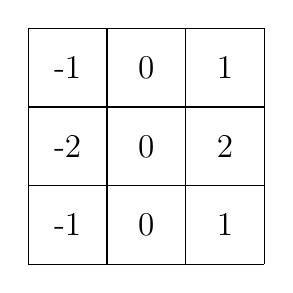
\begin{tikzpicture}
        \draw[step=1cm,color=black] (0, 0) grid (3,3);
        \node[font = {\large}, black] at (0.5, 2.5) {-1};
        \node[font = {\large}, black] at (1.5, 2.5) {0};
        \node[font = {\large}, black] at (2.5, 2.5) {1};
        \node[font = {\large}, black] at (0.5, 1.5) {-2};
        \node[font = {\large}, black] at (1.5, 1.5) {0};
        \node[font = {\large}, black] at (2.5, 1.5) {2};
        \node[font = {\large}, black] at (0.5, 0.5) {-1};
        \node[font = {\large}, black] at (1.5, 0.5) {0};
        \node[font = {\large}, black] at (2.5, 0.5) {1};
    \end{tikzpicture}
    \begin{tikzpicture}
        \draw[step=1cm,color=black] (1, 0) grid (2,3);

        \node[font = {\large}, black] at (1.5, 2.5) {1};


        \node[font = {\large}, black] at (1.5, 1.5) {2};


        \node[font = {\large}, black] at (1.5, 0.5) {1};

        
        \node[font = {\large}, black] at (-0.5, 1.5) {=};
    \end{tikzpicture}
    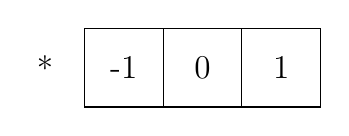
\begin{tikzpicture}
        \draw[step=1cm,color=black] (0, 2) grid (3,3);
        \node[font = {\large}, black] at (0.5, 2.5) {-1};


        \node[font = {\large}, black] at (1.5, 2.5) {0};


        \node[font = {\large}, black] at (2.5, 2.5) {1};

        
        \node[font = {\large}, black] at (-0.5, 2.5) {*};
    \end{tikzpicture}

\end{center}

\begin{center}
    Vertical Sobel filter, finds changes (edges) in x direction, thus vertical edges
\end{center}

\begin{center}
    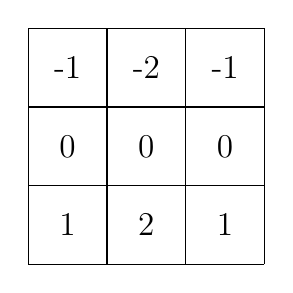
\begin{tikzpicture}
        \draw[step=1cm,color=black] (0, 0) grid (3,3);
        \node[font = {\large}, black] at (0.5, 2.5) {-1};
        \node[font = {\large}, black] at (1.5, 2.5) {-2};
        \node[font = {\large}, black] at (2.5, 2.5) {-1};
        \node[font = {\large}, black] at (0.5, 1.5) {0};
        \node[font = {\large}, black] at (1.5, 1.5) {0};
        \node[font = {\large}, black] at (2.5, 1.5) {0};
        \node[font = {\large}, black] at (0.5, 0.5) {1};
        \node[font = {\large}, black] at (1.5, 0.5) {2};
        \node[font = {\large}, black] at (2.5, 0.5) {1};
    \end{tikzpicture}
    \begin{tikzpicture}
        \draw[step=1cm,color=black] (1, 0) grid (2,3);

        \node[font = {\large}, black] at (1.5, 2.5) {-1};


        \node[font = {\large}, black] at (1.5, 1.5) {0};


        \node[font = {\large}, black] at (1.5, 0.5) {1};

        
        \node[font = {\large}, black] at (-0.5, 1.5) {=};
    \end{tikzpicture}
    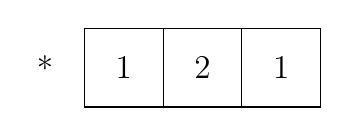
\begin{tikzpicture}
        \draw[step=1cm,color=black] (0, 2) grid (3,3);
        \node[font = {\large}, black] at (0.5, 2.5) {1};


        \node[font = {\large}, black] at (1.5, 2.5) {2};


        \node[font = {\large}, black] at (2.5, 2.5) {1};

        
        \node[font = {\large}, black] at (-0.5, 2.5) {*};
    \end{tikzpicture}

\end{center}

\begin{center}
    Horizontal Sobel filter, finds changes (edges) in y direction, thus horizontal edges
\end{center}

\newpage

\begin{itemize}
    \item \textbf{Horizontal Sobel filter} $\rightarrow$ when this filter is convolved with an image, it computes the horizontal gradient (it highlights the edges in the image that have a strong change in intensity in the horizontal direction); this means that it can be used to detect edges that are oriented horizontally in the image;
    \begin{center}
        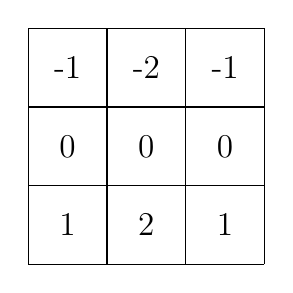
\begin{tikzpicture}
            \draw[step=1cm,color=black] (0, 0) grid (3,3);
            \node[font = {\large}, black] at (0.5, 2.5) {-1};
            \node[font = {\large}, black] at (1.5, 2.5) {-2};
            \node[font = {\large}, black] at (2.5, 2.5) {-1};
            \node[font = {\large}, black] at (0.5, 1.5) {0};
            \node[font = {\large}, black] at (1.5, 1.5) {0};
            \node[font = {\large}, black] at (2.5, 1.5) {0};
            \node[font = {\large}, black] at (0.5, 0.5) {1};
            \node[font = {\large}, black] at (1.5, 0.5) {2};
            \node[font = {\large}, black] at (2.5, 0.5) {1};
        \end{tikzpicture}
    \end{center}
    \item \textbf{Vertical Sobel filter} $\rightarrow$ when this filter is convolved with an image, it computes the vertical gradient (it highlights the edges in the image that have a strong change in intensity in the vertical direction); this means that it can be used to detect edges that are oriented vertically in the image;
    \begin{center}
        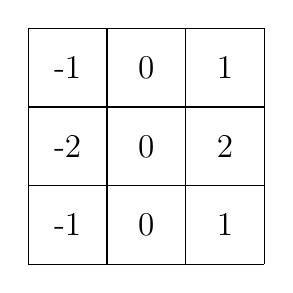
\begin{tikzpicture}
            \draw[step=1cm,color=black] (0, 0) grid (3,3);
            \node[font = {\large}, black] at (0.5, 2.5) {-1};
            \node[font = {\large}, black] at (1.5, 2.5) {0};
            \node[font = {\large}, black] at (2.5, 2.5) {1};
            \node[font = {\large}, black] at (0.5, 1.5) {-2};
            \node[font = {\large}, black] at (1.5, 1.5) {0};
            \node[font = {\large}, black] at (2.5, 1.5) {2};
            \node[font = {\large}, black] at (0.5, 0.5) {-1};
            \node[font = {\large}, black] at (1.5, 0.5) {0};
            \node[font = {\large}, black] at (2.5, 0.5) {1};
        \end{tikzpicture}
    \end{center}
\end{itemize}

In practice, these two filters are often used together in a technique called \textbf{Sobel edge detection}. By computing the magnitude of the gradient at each pixel using the horizontal and vertical Sobel filters, we can identify the regions in the image where there is a strong change in intensity in any direction, which are likely to correspond to edges in the image. \textbf{This is a rather naive technique}.

\newpage

\addcontentsline{toc}{section}{Other derivative filters}
\section*{Other derivative filters}

Depending on how you compute the distance between two pixels, the neighborhood size and so on, you can have different derivative filters:

\begin{center}
    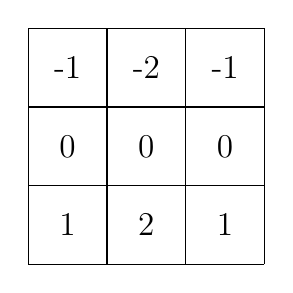
\begin{tikzpicture}
        \draw[step=1cm,color=black] (0, 0) grid (3,3);
        \node[font = {\large}, black] at (0.5, 2.5) {-1};
        \node[font = {\large}, black] at (1.5, 2.5) {-2};
        \node[font = {\large}, black] at (2.5, 2.5) {-1};
        \node[font = {\large}, black] at (0.5, 1.5) {0};
        \node[font = {\large}, black] at (1.5, 1.5) {0};
        \node[font = {\large}, black] at (2.5, 1.5) {0};
        \node[font = {\large}, black] at (0.5, 0.5) {1};
        \node[font = {\large}, black] at (1.5, 0.5) {2};
        \node[font = {\large}, black] at (2.5, 0.5) {1};
    \end{tikzpicture}
    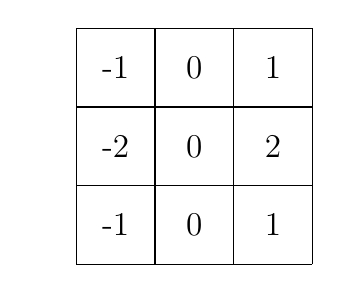
\begin{tikzpicture}
        \draw[step=1cm,color=black] (0, 0) grid (3,3);
        \node[font = {\large}, black] at (0.5, 2.5) {-1};
        \node[font = {\large}, black] at (1.5, 2.5) {0};
        \node[font = {\large}, black] at (2.5, 2.5) {1};
        \node[font = {\large}, black] at (0.5, 1.5) {-2};
        \node[font = {\large}, black] at (1.5, 1.5) {0};
        \node[font = {\large}, black] at (2.5, 1.5) {2};
        \node[font = {\large}, black] at (0.5, 0.5) {-1};
        \node[font = {\large}, black] at (1.5, 0.5) {0};
        \node[font = {\large}, black] at (2.5, 0.5) {1};

        \node[font = {\large}, black] at (-0.5, 1.5) {};
    \end{tikzpicture}
\end{center}

\begin{center}
    Horizontal and vertical Sobel filters
\end{center}

\begin{center}
    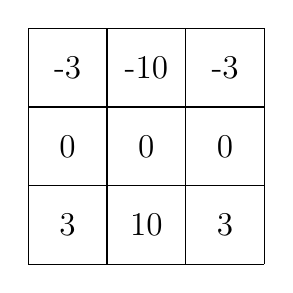
\begin{tikzpicture}
        \draw[step=1cm,color=black] (0, 0) grid (3,3);
        \node[font = {\large}, black] at (0.5, 2.5) {-3};
        \node[font = {\large}, black] at (1.5, 2.5) {-10};
        \node[font = {\large}, black] at (2.5, 2.5) {-3};
        \node[font = {\large}, black] at (0.5, 1.5) {0};
        \node[font = {\large}, black] at (1.5, 1.5) {0};
        \node[font = {\large}, black] at (2.5, 1.5) {0};
        \node[font = {\large}, black] at (0.5, 0.5) {3};
        \node[font = {\large}, black] at (1.5, 0.5) {10};
        \node[font = {\large}, black] at (2.5, 0.5) {3};
    \end{tikzpicture}
    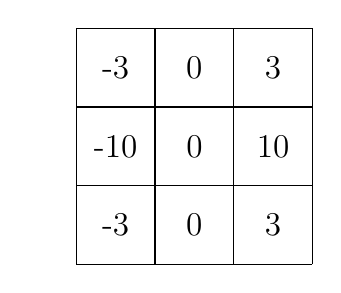
\begin{tikzpicture}
        \draw[step=1cm,color=black] (0, 0) grid (3,3);
        \node[font = {\large}, black] at (0.5, 2.5) {-3};
        \node[font = {\large}, black] at (1.5, 2.5) {0};
        \node[font = {\large}, black] at (2.5, 2.5) {3};
        \node[font = {\large}, black] at (0.5, 1.5) {-10};
        \node[font = {\large}, black] at (1.5, 1.5) {0};
        \node[font = {\large}, black] at (2.5, 1.5) {10};
        \node[font = {\large}, black] at (0.5, 0.5) {-3};
        \node[font = {\large}, black] at (1.5, 0.5) {0};
        \node[font = {\large}, black] at (2.5, 0.5) {3};

        \node[font = {\large}, black] at (-0.5, 1.5) {};
    \end{tikzpicture}
\end{center}

\begin{center}
    Horizontal and vertical Scharr filters
\end{center}

\begin{center}
    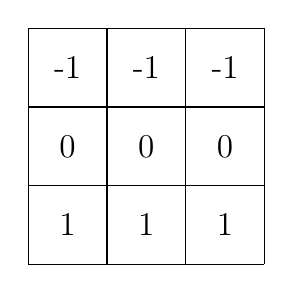
\begin{tikzpicture}
        \draw[step=1cm,color=black] (0, 0) grid (3,3);
        \node[font = {\large}, black] at (0.5, 2.5) {-1};
        \node[font = {\large}, black] at (1.5, 2.5) {-1};
        \node[font = {\large}, black] at (2.5, 2.5) {-1};
        \node[font = {\large}, black] at (0.5, 1.5) {0};
        \node[font = {\large}, black] at (1.5, 1.5) {0};
        \node[font = {\large}, black] at (2.5, 1.5) {0};
        \node[font = {\large}, black] at (0.5, 0.5) {1};
        \node[font = {\large}, black] at (1.5, 0.5) {1};
        \node[font = {\large}, black] at (2.5, 0.5) {1};
    \end{tikzpicture}
    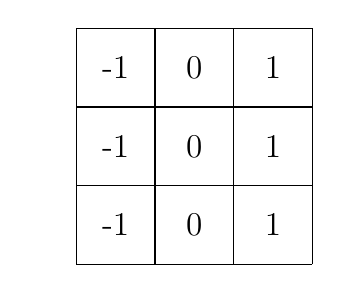
\begin{tikzpicture}
        \draw[step=1cm,color=black] (0, 0) grid (3,3);
        \node[font = {\large}, black] at (0.5, 2.5) {-1};
        \node[font = {\large}, black] at (1.5, 2.5) {0};
        \node[font = {\large}, black] at (2.5, 2.5) {1};
        \node[font = {\large}, black] at (0.5, 1.5) {-1};
        \node[font = {\large}, black] at (1.5, 1.5) {0};
        \node[font = {\large}, black] at (2.5, 1.5) {1};
        \node[font = {\large}, black] at (0.5, 0.5) {-1};
        \node[font = {\large}, black] at (1.5, 0.5) {0};
        \node[font = {\large}, black] at (2.5, 0.5) {1};

        \node[font = {\large}, black] at (-0.5, 1.5) {};
    \end{tikzpicture}
\end{center}

\begin{center}
    Horizontal and vertical Prewitt filters
\end{center}

\begin{center}
    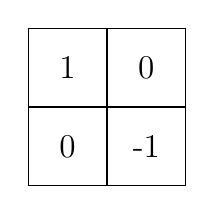
\begin{tikzpicture}
        \draw[step=1cm,color=black] (0, 0) grid (2,2);
        \node[font = {\large}, black] at (0.5, 1.5) {1};
        \node[font = {\large}, black] at (1.5, 1.5) {0};
        \node[font = {\large}, black] at (0.5, 0.5) {0};
        \node[font = {\large}, black] at (1.5, 0.5) {-1};
    \end{tikzpicture}
    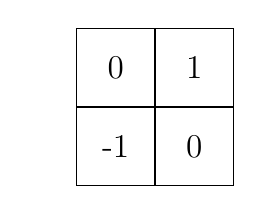
\begin{tikzpicture}
        \draw[step=1cm,color=black] (0, 0) grid (2,2);
        \node[font = {\large}, black] at (0.5, 1.5) {0};
        \node[font = {\large}, black] at (1.5, 1.5) {1};
        \node[font = {\large}, black] at (0.5, 0.5) {-1};
        \node[font = {\large}, black] at (1.5, 0.5) {0};

        \node[font = {\large}, black] at (-0.5, 1.5) {};
    \end{tikzpicture}
\end{center}

\begin{center}
    Horizontal and vertical Roberts filters
\end{center}

\newpage

\addcontentsline{toc}{section}{Computing image gradients}
\section*{Computing image gradients}

\begin{itemize}
    \item Select the derivative filters. In this example we will use the Sobel filter:
    \begin{center}
    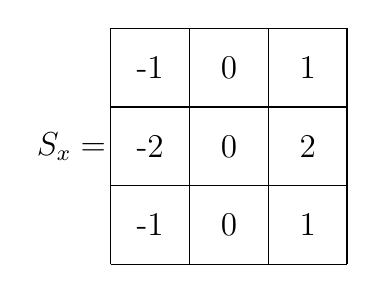
\begin{tikzpicture}
        \draw[step=1cm,color=black] (0, 0) grid (3,3);

        \node[font = {\large}, black] at (0.5, 2.5) {-1};
        \node[font = {\large}, black] at (1.5, 2.5) {0};
        \node[font = {\large}, black] at (2.5, 2.5) {1};
        \node[font = {\large}, black] at (0.5, 1.5) {-2};
        \node[font = {\large}, black] at (1.5, 1.5) {0};
        \node[font = {\large}, black] at (2.5, 1.5) {2};
        \node[font = {\large}, black] at (0.5, 0.5) {-1};
        \node[font = {\large}, black] at (1.5, 0.5) {0};
        \node[font = {\large}, black] at (2.5, 0.5) {1};

        \node[font = {\large}, black] at (-0.5, 1.5) {$S_x = $};

    \end{tikzpicture}
    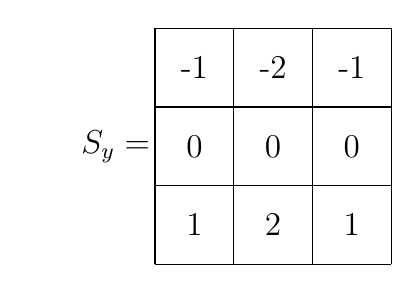
\begin{tikzpicture}
        \draw[step=1cm,color=black] (0, 0) grid (3,3);

        \node[font = {\large}, black] at (0.5, 2.5) {-1};
        \node[font = {\large}, black] at (1.5, 2.5) {-2};
        \node[font = {\large}, black] at (2.5, 2.5) {-1};
        \node[font = {\large}, black] at (0.5, 1.5) {0};
        \node[font = {\large}, black] at (1.5, 1.5) {0};
        \node[font = {\large}, black] at (2.5, 1.5) {0};
        \node[font = {\large}, black] at (0.5, 0.5) {1};
        \node[font = {\large}, black] at (1.5, 0.5) {2};
        \node[font = {\large}, black] at (2.5, 0.5) {1};

        \node[font = {\large}, black] at (-0.5, 1.5) {$S_y = $};

        \node[font = {\large}, black] at (-1.5, 1.5) {};
    \end{tikzpicture}
    \end{center}
    \item Convolve with the image to compute derivatives: \\ 
    
    \noindent\begin{minipage}{.5\linewidth}
    \begin{equation*}
        \frac{\partial f}{\partial x} = S_x \otimes f
    \end{equation*}
    \end{minipage}%
    \begin{minipage}{.5\linewidth}
    \begin{equation*}
        \frac{\partial f}{\partial y} = S_y \otimes f
    \end{equation*}
    \end{minipage}

    \item Form the image gradient and compute its direction and amplitude: \\

    \begin{equation*}
        \nabla f = \left[ \frac{\partial f}{\partial x}, \frac{\partial f}{\partial y} \right]        
    \end{equation*}
    \begin{center}
        Gradient
    \end{center}

    The gradient points in the direction of most rapid increase in intensity. The gradient direction and magnitude can be computed this way:

    \begin{equation*}
        \theta = \tan^{-1}{\left( \frac{\partial f}{\partial x} / \frac{\partial f}{\partial y} \right)}
    \end{equation*}
    \begin{center}
        Direction
    \end{center}

    \begin{equation*}
        \|\nabla f\| = \sqrt{\left( \frac{\partial f}{\partial x} \right)^2 + \left( \frac{\partial f}{\partial y} \right)^2}
    \end{equation*}
    \begin{center}
        Amplitude
    \end{center}
\end{itemize}

\newpage

\addcontentsline{toc}{section}{Using image gradients for edge detection}
\section*{Using image gradients for edge detection}

Given a signal

\begin{center}
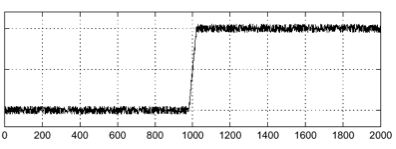
\includegraphics[width=0.8\textwidth]{images/signal.png}
\end{center}

Directly taking its derivative results in this:

\begin{center}
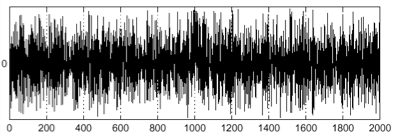
\includegraphics[width=0.8\textwidth]{images/derivative.png}
\end{center}

Blurring before taking the derivative:

\begin{center}
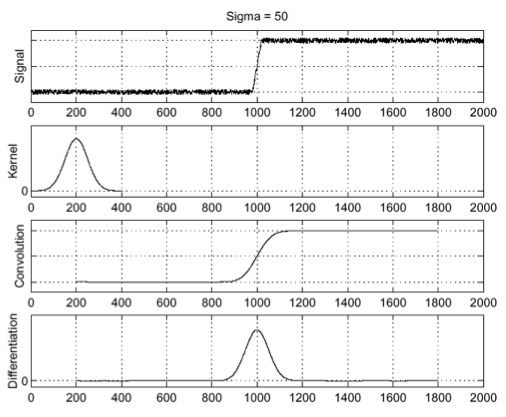
\includegraphics[width=0.8\textwidth]{images/blurring_before_derivation.png}
\end{center}

We can focus on peaks in the convolution between the image and a blurring filter to find edges.

\newpage

\addcontentsline{toc}{section}{Canny Edge detector}
\section*{Canny Edge detector}

The Canny Edge Detector is a technique that resorts on the gradient of the image to detect
edges. Edges correspond to a sudden change in pixel intensity. The algorithm requires the image
to be grayscale. It consists of 5 steps:

\begin{enumerate}[start=0]
    \item \textbf{Grayscale the image}.
    \item \textbf{Noise reduction}: resorting on the gradient, the pipeline is very susceptible to noise in the image, so the first step is to apply a Gaussian filter to blur it. We use the Gaussian over a Box filter for various reasons, first two among them are the fact that Box filter leaves ringing artifacts in the image and the fact that Gaussian filter better preserves the edges.
    \item \textbf{Gradient computation}: the smoothed image is then filtered with a Sobel kernel (first derivative) both in the horizontal direction ($G_x$) and in the vertical direction ($G_y$); once we have the image gradient we can compute the orientation and magnitude of the gradient at each pixel.
    \item \textbf{Non-maximum suppression}: ideally, the final image should have thin edges, thus we must perform non-maximum suppression to thin out the edges; the algorithm goes through all the points on the gradient intensity matrix and finds the pixels with the maximum value in the edge directions. The purpose of the algorithm is to check if the pixels on the same direction are more or less intense than the ones being processed. If the pixel (i, j) is being processed and the pixels on the same direction are (i, j-1) and (i, j+1), if one of those two pixels is more intense than the one being processed, then only the more intense one is kept.
    \item \textbf{Double threshold}: the double thresholding step is then applied to the resulting image with thin edges;
    it aims at identifying 3 kinds of pixels:
    \begin{itemize}
        \item \textbf{Strong pixels} are pixels that have an intensity so high that we are sure they contribute to the final edge;
        \item \textbf{Weak pixels} are pixels that have an intensity value that is not enough to be considered as strong ones, but yet not small enough to be considered as nonrelevant for the edge detection;
        \item Other pixels are considered as \textbf{non-relevant} for the edge.
    \end{itemize}
    The threshold values are chosen empirically.
    \item \textbf{Linking}: based on the threshold results, the linking consists in transforming weak pixels into strong ones if and only if at least one of the pixels around the one being processed is a strong one.
\end{enumerate}

Threshold and linking steps are also referred to as hysteresis.

\newpage

\addcontentsline{toc}{section}{Non-maximum suppression}
\section*{Non-maximum suppression}

Non-maximum suppression is performed to thin out the edges to a single pixel in width; the algorithm goes through all the points on the gradient intensity matrix and finds the pixels with the maximum value in the edge directions. The purpose of the algorithm is to check if the pixels on the same direction are more or less intense than the ones being processed.

\vspace{2cm}

\begin{center}
    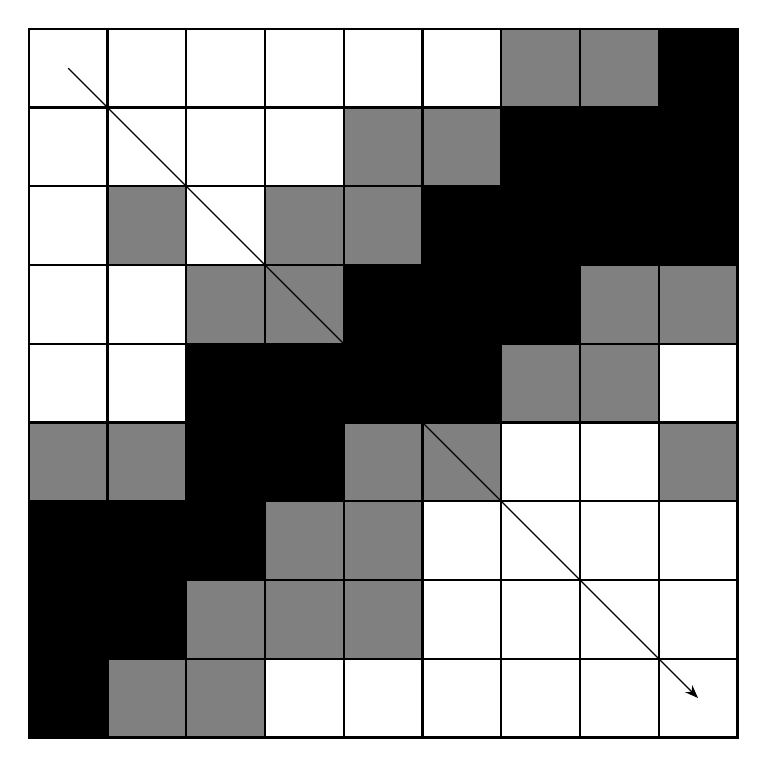
\begin{tikzpicture}
        [
            box/.style={rectangle,draw=black,thick, minimum size=1cm},
        ]
    
    \foreach \x [count=\i from 0] in {0,1,...,8}
        \foreach \y [count=\j from 0] in {0,1,...,8}
        {
            \def\bit{0}
                \pgfmathsetmacro{\bit}{\pixelmap[\i][\j]}
            %\draw[grid] (\x,-2.5) -- (\x,2.5);
            %\draw[grid] (-2.5,\y) -- (2.5,\y);
            %\fill[cube, color\bit] (\x,\y) -- +(0, 0.25) -- +(.25, .25) -- +(.25,0) -- cycle;
            
            \node[box,fill=color\bit] at (\x, \y) {};
        }

    \draw[-{Stealth[black]}] (0, 8) -- (8, 0);
    
    \end{tikzpicture}
\end{center}

\newpage

\addcontentsline{toc}{section}{Laplace filter}
\section*{Laplace filter}

Laplace filter is a \textbf{second derivative filter}. \\

The first-order finite difference

\begin{center}
    \begin{equation*}
        f'(x) = \lim_{h\to 0} \frac{f(x + 0.5h) - f(x - 0.5h)}{h}
    \end{equation*}
\end{center}

results in a 1D derivative filter:

\begin{center}
    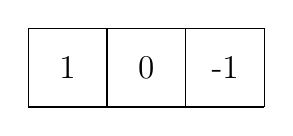
\begin{tikzpicture}
        \draw[step=1cm,color=black] (0, 2) grid (3,3);
        \node[font = {\large}, black] at (0.5, 2.5) {1};
        \node[font = {\large}, black] at (1.5, 2.5) {0};
        \node[font = {\large}, black] at (2.5, 2.5) {-1};
    \end{tikzpicture}
\end{center}

\vspace{0.5cm}

The second-order finite difference

\begin{center}
    \begin{equation*}
        f''(x) = \lim_{h\to 0} \frac{f(x + h) - 2f(x) + f(x - h)}{h^2}
    \end{equation*}
\end{center}

results in a 1D Laplace filter:

\begin{center}
    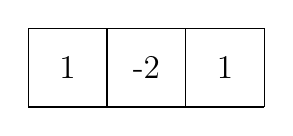
\begin{tikzpicture}
        \draw[step=1cm,color=black] (0, 2) grid (3,3);
        \node[font = {\large}, black] at (0.5, 2.5) {1};
        \node[font = {\large}, black] at (1.5, 2.5) {-2};
        \node[font = {\large}, black] at (2.5, 2.5) {1};
    \end{tikzpicture}
\end{center}

\hspace{2cm}

\begin{center}
    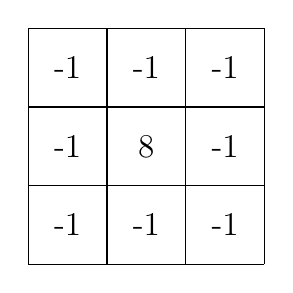
\begin{tikzpicture}
        \draw[step=1cm,color=black] (0, 0) grid (3,3);
        \node[font = {\large}, black] at (0.5, 2.5) {-1};
        \node[font = {\large}, black] at (1.5, 2.5) {-1};
        \node[font = {\large}, black] at (2.5, 2.5) {-1};
        \node[font = {\large}, black] at (0.5, 1.5) {-1};
        \node[font = {\large}, black] at (1.5, 1.5) {8};
        \node[font = {\large}, black] at (2.5, 1.5) {-1};
        \node[font = {\large}, black] at (0.5, 0.5) {-1};
        \node[font = {\large}, black] at (1.5, 0.5) {-1};
        \node[font = {\large}, black] at (2.5, 0.5) {-1};
    \end{tikzpicture}
    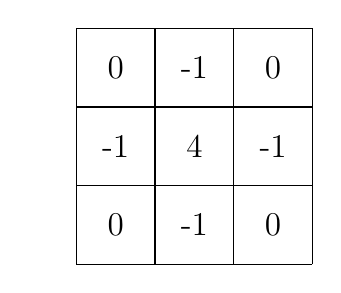
\begin{tikzpicture}
        \draw[step=1cm,color=black] (0, 0) grid (3,3);
        \node[font = {\large}, black] at (0.5, 2.5) {0};
        \node[font = {\large}, black] at (1.5, 2.5) {-1};
        \node[font = {\large}, black] at (2.5, 2.5) {0};
        \node[font = {\large}, black] at (0.5, 1.5) {-1};
        \node[font = {\large}, black] at (1.5, 1.5) {4};
        \node[font = {\large}, black] at (2.5, 1.5) {-1};
        \node[font = {\large}, black] at (0.5, 0.5) {0};
        \node[font = {\large}, black] at (1.5, 0.5) {-1};
        \node[font = {\large}, black] at (2.5, 0.5) {0};

        \node[font = {\large}, black] at (-0.5, 1.5) {};
    \end{tikzpicture}
\end{center}

\begin{center}
    Laplacian operator with and without diagonals
\end{center}

\newpage

\addcontentsline{toc}{section}{Laplacian of Gaussian (LoG) filter}
\section*{Laplacian of Gaussian (LoG) filter}

Instead of convolving the image with the kernel and \textbf{then} taking the derivative (expensive operation since the derivative is taken with respect to the whole image), we can first compute the derivative of the filter (small) and then convolve it with the image. \\

We obtain this:
\begin{center}
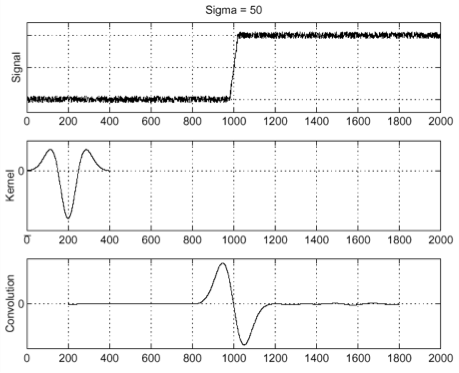
\includegraphics[width=0.8\textwidth]{images/laplacian_derivative.png}
\end{center}

With the second derivative (laplacian) we have a \textbf{zero-crossing behaviour at edges}, whilst in with the first derivative we had a peak in the same spot. It is \textbf{easier to search for a zero} than to find a maximum.

Building off of this procedure we can design an edge detector.

\newpage

\addcontentsline{toc}{section}{Naive Image Downsampling}
\section*{Naive Image Downsampling}

\textbf{How could we reduce the image size?} A naive approach could be to throw away half the rows and/or columns. \textbf{Why half? Is it enough?} Images are a discrete, sampled, representation of a continuous world. If you undersample the image, like any other kind of signal, you won't be able to reconstruct it without information loss. \\

Consider a very simple example, a sine wave:

\begin{center}
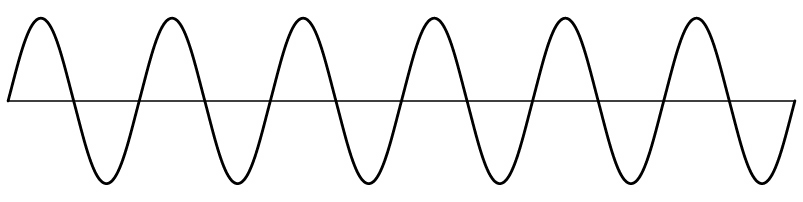
\includegraphics[width=0.8\textwidth]{images/signal_2.png}
\end{center}

Suppose you sample the signal like so:

\begin{center}
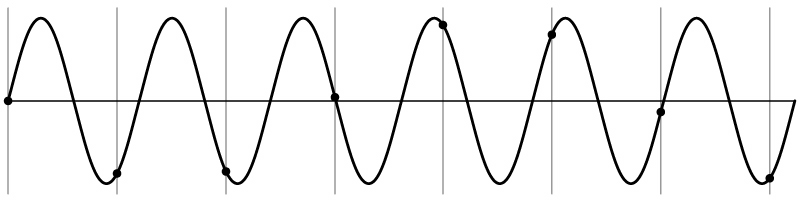
\includegraphics[width=0.8\textwidth]{images/undersampling.png}
\end{center}

When you try to reconstruct the signal, you can confuse it with one of lower frequency:

\begin{center}
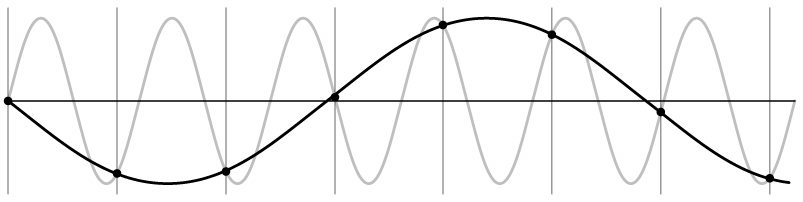
\includegraphics[width=0.8\textwidth]{images/undersampling_lower_freq.png}
\end{center}

Note that we could always confuse the signal with one of higher frequency even if we sample correctly:

\begin{center}
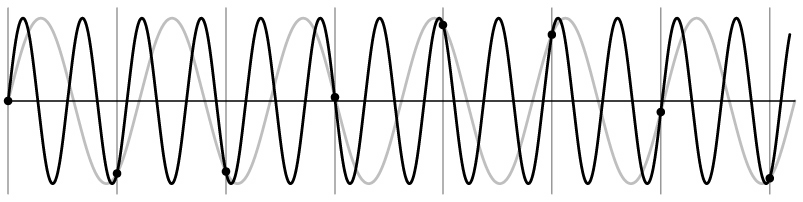
\includegraphics[width=0.8\textwidth]{images/undersampling_higher_freq.png}
\end{center}

\newpage

\textbf{We have undersampling when we can disguise a signal as one of lower frequency}. The resulting effect is called \textbf{aliasing}. \\

The \textbf{Nyquist sampling theory} states that the sample rate needs to be at least 2 times the highest frequency component (cutoff frequency) of your input signal to prevent aliasing; that rate is called \textbf{Nyquist rate}. Aliasing is a phenomenon where higher frequency components fold back into your signal and cause interference.

\addcontentsline{toc}{section}{How to deal with aliasing?}
\section*{How to deal with aliasing?}

\begin{itemize}
    \item \textbf{Oversample the signal}: you should sample with a rate over the Nyquist rate.
    \item \textbf{Smooth the signal}: remove some of the details that cause aliasing; this causes information loss but lets you have better aliasing artifacts. 
\end{itemize}

Dealing with images, we can apply a smoothing filter (Gaussian, box, ...) first, then proceed to downsample (throw away half the rows and columns). \\

How much smoothing do we need to avoid aliasing? How many samples do we need to avoid aliasing? \textbf{Enough to reach the Nyquist limit of 2 times the highest frequency reached by the image}. How can we practically reduce aliasing? By smoothing the signal we remove high frequency components (features) and thus lower the Niquist rate ($\geq$ two times the maximum frequency).

\newpage

\addcontentsline{toc}{section}{Gaussian Image Pyramid}
\section*{Gaussian Image Pyramid}

Image pyramids are a type of multi-scale representation of an image, where the original image is successively down-sampled to create a series of smaller versions, each representing a different level of detail. They are important because they allow us to perform operations such as object detection, feature extraction, and image segmentation at multiple scales, which can be useful in a variety of computer vision applications.

\begin{itemize}
    \item \textbf{Multi-scale image analysis}: By using image pyramids, we can process an image at different scales, allowing us to detect objects or features that may appear at different sizes in the image. This can be useful in scenarios where the size of an object in the image is not known in advance, or when we need to detect objects or features that may have different sizes in different parts of the image.
    \item \textbf{Feature extraction}: Image pyramids can be used for feature extraction, where we extract features from the different levels of the pyramid and use them to represent the image at multiple scales. This can be useful in tasks such as image classification, where we want to use features that capture different levels of detail in the image.
    \item \textbf{Image blending}: Image pyramids can be used for image blending, where we combine two images of different sizes or resolutions. By constructing image pyramids for each image, we can blend them at different levels of the pyramid to create a seamless blend between the images.
\end{itemize}

Overall, image pyramids are an important tool in computer vision and image processing, allowing us to process images at multiple scales and extract features that capture different levels of detail. \\

Image pyramids allow us to perform operations on images at different resolutions, which can be \textbf{computationally efficient}. For example, instead of processing the original image at high resolution, we can first down-sample the image and then perform the operation on the smaller image, reducing the computational cost. All this at what cost? How much is the image pyramid bigger than the original image? \textbf{The whole image pyramid is just $4/3$ times the size of the original image}. 

\newpage

\addcontentsline{toc}{section}{Laplacian Image Pyramid}
\section*{Laplacian Image Pyramid}

Going up a level in a Gaussian Image Pyramid we loose features, high frequency components. Mostly large uniform regions are preserved. It is not possible to reconstruct the original image from the image at the upper level in the pyramid alone. This is why we introduce the \textbf{Laplacian Image Pyramid}. \\

The Laplacian pyramid is constructed by decomposing the original image into a series of bandpass-filtered images, where each image is obtained by subtracting the upsampled version of the next level's image from the current level's image. This difference image is also called \textbf{residual}, as it represents the high-frequency details or edges in the image that were removed by the bandpass filtering. \\

The Laplacian pyramid is typically constructed by first computing a Gaussian pyramid and then subtracting the upsampled version of each Gaussian pyramid level from the next level in the Gaussian pyramid. \\

Thus, we have both the residual image, which contains the high-frequency details or edges that were removed during the Gaussian filtering, and the downsampled images, which contain the low-frequency information. By storing both the residual and downsampled images we have a multi-scale representation of the image that can be used for tasks such as image compression, feature extraction, and image blending.

\begin{center}
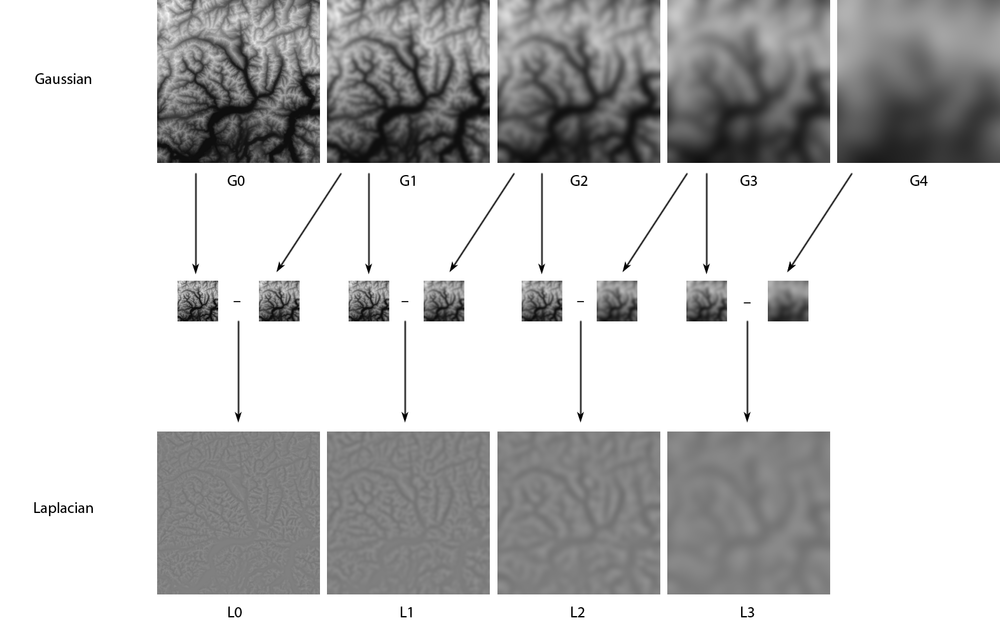
\includegraphics[width=0.95\textwidth]{images/pyramids.png}
\end{center}

\newpage

\addcontentsline{toc}{section}{Constructing a Laplacian Pyramid}
\section*{Constructing a Laplacian Pyramid}

The $k$-th level of Laplacian pyramid can be obtained by the following formula:

\begin{equation*}
    L_k(I) = G_k(I) - u(G_{k+1}(I))
\end{equation*}

\begin{center}
    \textit{$I$ is the input image} \\
    \textit{$L_k(I)$ is the $k$-th level of the Laplacian pyramid} \\
    \textit{$G_k(I)$ is the $k$-th level of the Gaussian pyramid} \\
    \textit{$u(\cdot)$ is a 2x scale-up operation}
\end{center}

These are the steps to build a Laplacian pyramid:
\begin{enumerate}
    \item Create a Gaussian image pyramid. The Gaussian pyramid is computed by repeatedly applying a Gaussian filter to the image and then down-sampling it.
    \item Create a Laplacian image pyramid by subtracting an up-sampled and blurred version of the image from the original image at each level of the pyramid. To do this, follow these steps:
    \begin{itemize}
        \item Starting with the higher level of the Gaussian pyramid ($k + 1$ if we are on level $k$), up-sample it.
        \item Apply a Gaussian filter to the up-sampled image.
        \item Subtract the resulting blurred image from the corresponding level of the Gaussian pyramid to get the Laplacian image.        
    \end{itemize}
    \item Repeat step 2 for all levels of the Gaussian pyramid, except the lowest level, which does not have a corresponding lower level to subtract from.
\end{enumerate}

\newpage

\begin{minted}
[
bgcolor=white,
fontsize=\footnotesize,
linenos
]
{python}
levels = 3

# Create a Gaussian Pyramid
lower = img.copy()
gaussian_pyr = [lower]
for i in range(levels):
   lower = cv2.pyrDown(lower)
   gaussian_pyr.append(lower)

# Last level of Gaussian remains same in Laplacian
laplacian_top = gaussian_pyr[-1]

# Create a Laplacian Pyramid
laplacian_pyr = []
for i in range(levels,0,-1):
   size = (gaussian_pyr[i - 1].shape[1], gaussian_pyr[i - 1].shape[0])
   gaussian_expanded = cv2.pyrUp(gaussian_pyr[i], dstsize=size)
   laplacian = cv2.subtract(gaussian_pyr[i-1], gaussian_expanded)
   laplacian_pyr.append(laplacian)

plot_all(gaussian_pyr, ['Gaussian ({})'.format(i) for i in range(len(gaussian_pyr))])
plot_all(laplacian_pyr, ['Laplacian ({})'.format(i) for i in range(len(laplacian_pyr))])
\end{minted}

\begin{center}
    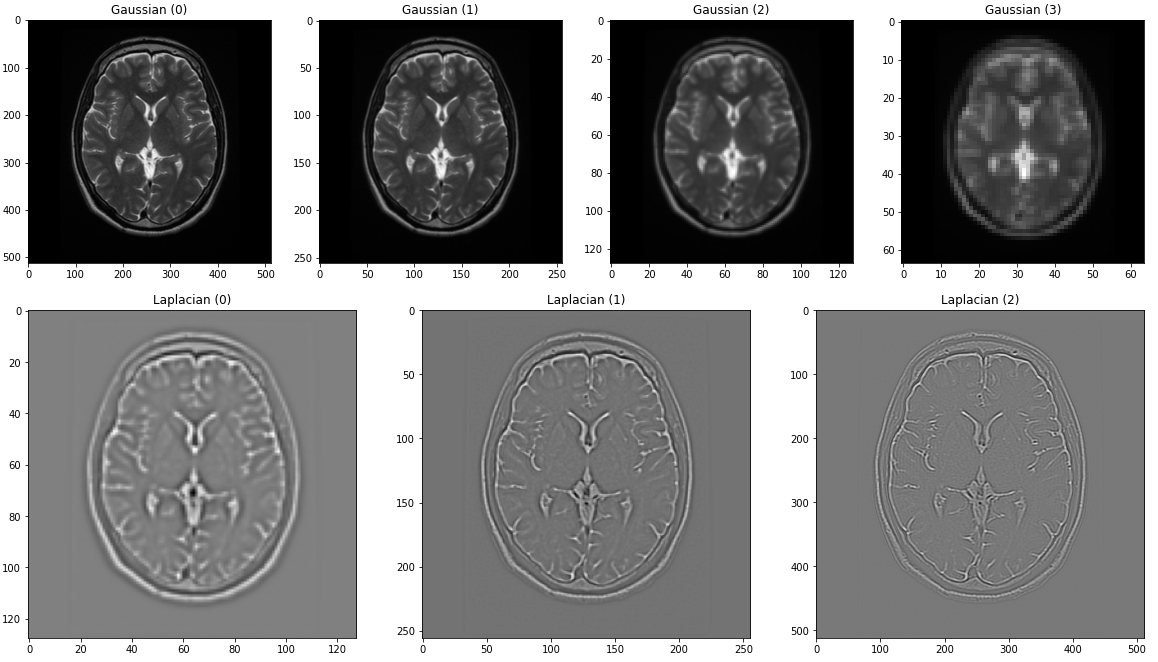
\includegraphics[width=0.95\textwidth]{images/pyr_example.png}
\end{center}

\newpage

\addcontentsline{toc}{section}{Steerable pyramid}
\section*{Steerable pyramid}

A steerable pyramid is a type of image decomposition algorithm that can be used for tasks such as image compression, feature extraction, and object recognition.

The basic idea behind a steerable pyramid is to construct a series of filters that can be applied to the image at different scales and orientations. The filters are designed in such a way that they can be steered in any direction, which means that they can be rotated to match the orientation of the features in the image. This allows the steerable pyramid to capture information in a directionally selective way, which is useful for tasks such as edge detection or texture analysis.

The steerable pyramid can be constructed using a set of bandpass filters that are applied to the image at different scales and orientations. The filters are typically implemented using a wavelet transform, which decomposes the image into a series of frequency bands. Each frequency band is then convolved with a set of filters that are steerable in different directions.

Once the steerable pyramid is constructed, it can be used for a variety of image processing tasks. For example, the pyramid can be used for image compression by discarding the high-frequency subbands, which contain fine details that are not essential for reconstructing the image. The pyramid can also be used for feature extraction by analyzing the responses of the different subbands to detect edges, corners, or other features in the image.

\newpage

\addcontentsline{toc}{section}{Image frequency}
\section*{Image frequency}

We can easily think about audio signals as sound waves varying at certain frequencies. High-frequency is a high pitched noise, like a bird chirp, while low frequency sounds are low pitch, like a deep voice or a bass drum. For sound, frequency actually refers to how fast a sound wave is oscillating. As for sound, frequency in images is a rate of change. While sound varies across time, images varies across space. An high frequency image is one where the intensity of pixels changes a lot, a low frequency image may be one that is relatively uniform in brightness or changes very slowly. \\

The Fourier Transform (FT) is an important image processing tool which is used to decompose an image into its frequency components. The output of an FT represents the image in the frequency domain, while the input image is the spatial domain (x, y) equivalent. In the frequency domain image, each point represents a particular frequency contained in the spatial domain image. So, for images with a lot of high-frequency components (edges, corners, and stripes), there will be a number of points in the frequency domain at high frequency values.

\addcontentsline{toc}{section}{Fourier Series}
\section*{Fourier Series}

The Fourier theorem state that any univariate function (signal) can be expressed as a weighted sum of sines and cosines of various frequencies. 

\begin{equation*}
    A \sin(\omega x + \phi) 
\end{equation*}

Basically, if we add enough of these blocks we can build any periodic signal we want. This thing also works for non-periodic signals, as long as the area under the curve is finite.

\addcontentsline{toc}{section}{Fourier Transform}
\section*{Fourier Transform}

The mathematical tool used to do this is known as the Fourier Transform:

\begin{equation*}
    f(x) = \int_{-\infty}^{\infty}F(k) e^{j2\pi kx}dk
\end{equation*}

This is used for continuous signals. What about images? Well, as for sound, frequency in images is a \textbf{rate of change}. So, what does it means for an image to change? Differently from sound, which varies across time, \textbf{images change in space}.

\begin{itemize}
    \item a \textbf{high frequency image} is one where the intensity of pixels changes a lot;
    \item a \textbf{low frequency image} may be one that is relatively uniform in brightness or changes very slowly;
\end{itemize}

For discrete signals we will use the discrete Fourier Transform:
\begin{equation*}
    f(x) = \sum_{k=0}^{N-1} F(x) e^{j2\pi kx / N}
\end{equation*}

Being images 2D, we use a 2D Fourier Transform:
\begin{equation*}
    f(x,y) = \frac{1}{MN}\sum_{u=0}^{M-1} \sum_{v=0}^{N-1} F(u, v) e^{-j2\pi(ux/M + vy/N)}
\end{equation*}

The \textbf{Fourier Transform (FT)} is an important image processing tool which is used to decompose an image into its frequency components. The output of a Fourier Transform represents the image in the frequency domain, while the input image is the spatial domain (x, y) equivalent. In the frequency domain image, each point represents a particular frequency contained in the spatial domain image. So, for images with a lot of high-frequency components (edges, corners, and stripes), there will be a number of points in the frequency domain with high frequency values. \textbf{Zero frequency component (DC component) will be at top left corner}. DC components are shifted on the center for ease of visualization, obtaining the \textbf{frequency transform image}.\\ 

In practice, this is implemented by using the \textbf{fast Fourier Transform (FFT)} algorithm.

\newpage

\addcontentsline{toc}{section}{Convolution theorem}
\section*{Convolution theorem}

The Fourier Transform of the convolution of two functions is the product of their Fourier transforms:

\begin{equation*}
    F(g * h) = F(g)F(h)
\end{equation*}

The inverse Fourier Transform of the product of two functions is the convolution of the inverse of the Fourier transforms of the two functions:

\begin{equation*}
    F^{-1}(gh) = F^{-1}(g) * F^{-1}(h)
\end{equation*}

\textbf{Convolution in spatial domain is equivalent to multiplication in frequency domain}. Using the convolution theorem, we can implement all types of linear shift-invariant filtering as multiplication in the frequency domain (basically multiply the image with a mask).

\addcontentsline{toc}{section}{Blurring in frequency domain}
\section*{Blurring in frequency domain}

\begin{itemize}
    \item Low frequencies are in the middle of the frequency transform image.
    \item High frequencies are far from the center of the frequency transform image. 
\end{itemize}

Blurring an image involves attenuating or filtering out high-frequency components. The goal is to reduce image noise and/or to reduce the level of detail in the image. In the frequency domain, high-frequency components are far from the center of the image. To apply blurring in the frequency domain, a low-pass filter is needed. The low-pass filter attenuates high-frequency components and preserves low-frequency components. A simple example of a low-pass filter is the Gaussian filter, which has a bell-shaped response that attenuates high-frequency components. Another example is the square filter.

\begin{center}
    \begin{tabular}{lll}
        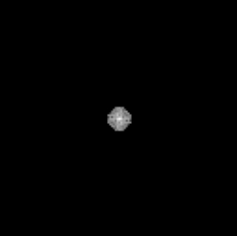
\includegraphics[width=.3\linewidth]{images/low_pass.jpg} &   
        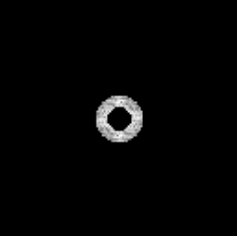
\includegraphics[width=.3\linewidth]{images/band_pass.jpg} &
        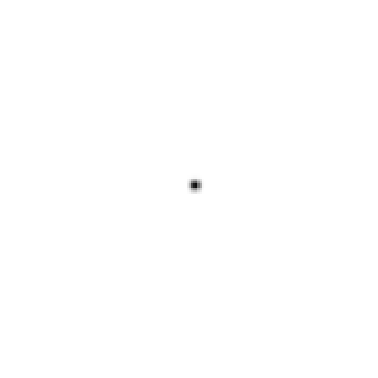
\includegraphics[width=.3\linewidth]{images/high_pass.png} \\
        \hspace{0.2cm} \\
        \text{Low-pass} &
        \text{Band-pass} &
        \text{High-pass} \\
    \end{tabular}
\end{center}

\newpage

\addcontentsline{toc}{section}{Gaussian vs Box filter in frequency domain}
\section*{Gaussian vs Box filter in frequency domain}

Both the Gaussian and the Box filter are low-pass filters. \\

\begin{center}
    \begin{tabular}{ll}
        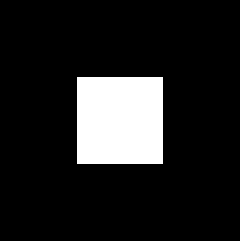
\includegraphics[width=.4\linewidth]{images/box_freq.jpg} &
        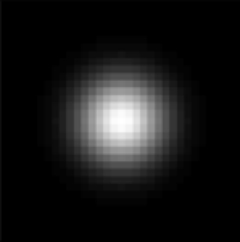
\includegraphics[width=.4\linewidth]{images/gaussian_freq.jpg} \\
        \hspace{0.2cm} \\
        \text{Box} &
        \text{Gaussian} \\
    \end{tabular}
\end{center}

In the frequency domain, the Fourier Transform of a Box filter is a sinc function, which has a main lobe with significant energy and high sidelobes that decay slowly. The sinc function has a narrow bandwidth, which means that it preserves high-frequency content. \\

On the other hand, the Fourier Transform of a Gaussian filter is also a Gaussian function that has a wider bandwidth than the sinc function of the Box filter. This means that the Gaussian filter attenuates high-frequency components more than the Box filter. \\

Compared to the Box filter, the \textbf{Gaussian filter} is more effective at \textbf{reducing high-frequency noise while preserving edges and details} in the image. This is because the Gaussian filter has a smooth, bell-shaped response that preserves more spatial information than the sharp, rectangular response of the Box filter. Furthermore the \textbf{box filter introduces ringing}. The ringing effect appears as oscillations or ripples around edges and sharp transitions in the image, which can make the image appear distorted or blurry. The sidelobes of the sinc function (Fourier Transform of the box filter) are responsible for the ringing effect because they spread the energy of the signal into neighboring frequencies, causing oscillations around sharp transitions.

\newpage

\addcontentsline{toc}{section}{Ideal Low Pass Filter (ILPF)}
\section*{Ideal Low Pass Filter (ILPF)}

An \textbf{ideal low-pass filter (ILPF)} is defined by:

\begin{equation*}
    H(u, v) = \begin{cases}
      1 if D(u,v) \leq D_0\\
      0 if D(u,v) > D_0
    \end{cases}
\end{equation*}

The point of transition between $H(u,v) = 1$ and $H(u,v) = 0$ is called \textbf{cutoff frequency}. \\

An ideal low-pass filter is a theoretical filter that completely eliminates all frequencies above a certain cutoff frequency while allowing all frequencies below that cutoff to pass through unaffected. \\

In an ideal low-pass filter, there is no attenuation of the desired frequencies below the cutoff frequency, and no distortion or delay of the signals passing through the filter. Additionally, the filter has an infinite roll-off, meaning that it provides complete attenuation of all frequencies above the cutoff frequency with no ripple in the passband. \\

It is impossible to build a real-world low-pass filter for various reasons:
\begin{itemize}
    \item The components used in the construction of a filter, such as resistors, capacitors, and inductors, have inherent limitations in their performance characteristics. For example, capacitors have a limited frequency response, while inductors have resistance, which can limit their effectiveness at high frequencies.
    \item The signal processing techniques used to implement a low-pass filter, such as digital signal processing or analog signal processing, are subject to limitations in their precision and accuracy. These limitations can result in errors in the filtering process, which can affect the quality of the output signal.
\end{itemize}

But while this thing applies to analog components, why can't we simulate it with an algorithm?
\begin{itemize}
    \item An ideal low pass filter has an \textbf{Infinite Impulse Response (IIR)}, which means that it requires an infinite number of computations to be implemented. In practice, only \textbf{Finite Impulse Response (FIR)} filters can be implemented, which have a limited number of coefficients and are therefore unable to achieve the ideal low pass filter response.
\end{itemize}

While \textbf{an ideal low-pass filter cannot be achieved in practice}, various types of real-world low-pass filters, such as Butterworth, Chebyshev, and Bessel filters, are designed to approximate the ideal response as closely as possible within certain design constraints. \\

\newpage

\addcontentsline{toc}{section}{Invariant local features}
\section*{Invariant local features}

In image processing, \textbf{local features} refer to distinctive patterns or structures in an image that can be used to identify and describe specific regions of the image. Local features are typically extracted from an image by \textbf{analyzing small regions of the image, rather than the image as a whole}. This approach is known as \textbf{local analysis}. \\

We obviously want to find features that are invariant to transformations:
\begin{itemize}
    \item \textbf{geometric invariance}: translation, rotation, scale, ...
    \item \textbf{photometric invariance}: brightness, exposure, ... 
\end{itemize}

Examples of local features include: 
\begin{itemize}
    \item \textbf{Corner features} are points where the image intensity changes in multiple directions;
    \item \textbf{Blob features} are regions of the image with a distinct shape or texture;
    \item \textbf{Edge features} are areas where the intensity changes abruptly in one direction;
    \item \textbf{Texture features} describe repeating patterns or structures in the image;
\end{itemize}

Once local features have been identified and extracted (\textbf{feature extraction}) from an image, they can be used to create a feature vector that describes the image (\textbf{feature description}). This feature vector can then be used for tasks such as object recognition or image matching, by comparing the features of different images and identifying those that are most similar.

\addcontentsline{toc}{section}{Why extract features?}
\section*{Why extract features?}

\begin{itemize}
    \item \textbf{Panorama stitching}: combine two or more images;
    \item \textbf{Visual SLAM}: constructing and updating a map of an unknown environment while simultaneously keeping track of an agent's location in it;
    \item \textbf{Image matching};
\end{itemize}

\addcontentsline{toc}{section}{Corner Detection}
\section*{Corner Detection}

\textbf{Corners are points in an image where the intensity or color changes significantly in multiple directions}, and they are often associated with the intersection of edges or contours in an image. By detecting these corners, we can identify the locations of objects and their boundaries in an image, as well as extract important information.

\newpage

\addcontentsline{toc}{section}{Harris Corner Detector - Mathematical Formulation}
\section*{Harris Corner Detector - Mathematical Formulation}

\textbf{A corner is a point whose local neighborhood is characterized by large intensity variation in multiple directions}, and they are considered as important features of an image since \textbf{they are scale invariant}. They are often used in various computer vision and image processing tasks such as object recognition, image registration, and image matching. \textbf{Harris Corner Detector is a frequently used technique} in computer vision and one of the first takes to tackle the corner detection problem. For more information on the Harris Corner Detector (emphasis on the relation between eigenvalues and the ellipsoid containing the points) you can check \href{https://guangchun.wordpress.com/2013/02/16/harris-detector/}{here}. \\

Consider a two-dimensional image $I$ and a patch $W$ of size $m \times m$ centered in $(x_0, y_0)$. We want to evaluate the intensity variation occurred if the window $W$ is shifted by a small amount $(u, v)$. Such variation can be estimated by computing the \textbf{Sum of Squared Differences (SSD)}:

\begin{equation*}
    SSD(u, v) = \sum_{(x,y)}g(x,y)[I(x,y) - I(x+u, y+v)]^2
\end{equation*}

Where $g(x,y)$ is a window function that only enables the pixels in the window. We need to maximize the function $SSD(u,v)$ for corner detection, thus finding the windows (and their centers) in which the intensity variation is maximum. Since $u$ and $v$ are small, the shifted intensity $I(x+u, y+v)$ can be approximated by the first-order Taylor expansion:

\begin{equation*}
    I(x+u, y+v) \approx I(x,y) + uI_x(x,y) + vI_y(x,y)
\end{equation*}

Where $I_x$ and $I_y$ are partial derivatives of $I$ in $x$ and $y$ direction respectively. We obtain:

\begin{equation*}
    \begin{split}
        SSD(u, v) & = \sum_{(x,y) \in W}[I(x,y) - I(x+u, y+v)]^2 \\ & \approx \sum_{(x,y) \in W}g(x,y)[I(x,y) - (I(x,y) + uI_x(x,y) + vI_y(x,y))]^2 \\
        & \approx \sum_{(x,y) \in W}[I(x,y) - I(x,y) + \begin{bmatrix} I_x & I_y \end{bmatrix} \begin{bmatrix} u \\ v \end{bmatrix}]^2 \\
        & \approx \sum_{(x,y) \in W}[\begin{bmatrix} I_x & I_y \end{bmatrix} \begin{bmatrix} u \\ v \end{bmatrix}]^2 \\
        & \approx \sum_{(x,y) \in W}[u^2I_x^2+2uvI_xI_y+v^2I_y^2]
    \end{split}
\end{equation*}

\newpage

\begin{equation*}
    \begin{split}
        SSD(u, v) & \approx \sum_{(x,y) \in W} [u^2I_x^2+2uvI_xI_y+v^2I_y^2] \\
        & \approx Au^2 + 2Buv + Cv^2
    \end{split}
\end{equation*}

With $A = \sum_{(x,y) \in W}I_x^2$, $B = \sum_{(x,y) \in W}I_xI_y$ and $C = \sum_{(x,y) \in W}I_y^2$. \\

This equation can be expressed in the following matrix form:

\begin{equation*}
SSD(u,v) \approx \begin{bmatrix} u & v \end{bmatrix} M 
\begin{bmatrix} u \\ v \end{bmatrix} 
\end{equation*}

Where $M$ is a $2 \times 2$ matrix computed from image derivatives:

\begin{equation*}
    M = \sum_{(x,y)}g(x,y)\begin{bmatrix} I_xI_x & I_xI_y \\ I_xI_y & I_yI_y\end{bmatrix}
\end{equation*}

This matrix is called \textbf{structure tensor} or \textbf{second moment matrix}. \\

The surface $E(u,v)$ is locally approximated by a quadratic form

\begin{center}
    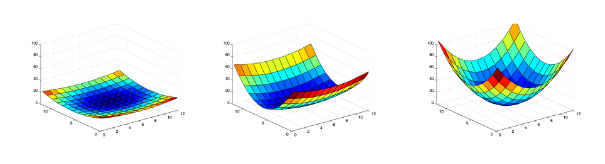
\includegraphics[width=.95\linewidth]{images/quadratic.png}    
\end{center}

From left to right, the error surface indicates a flat area, an edge and a corner. \\

The Harris detector uses the following response function (\textbf{Harris response function}) that scores the presence of a corner within the patch:

\begin{equation*}
    R = det(M) - k\ tr(M)^2
\end{equation*}

$k$ is an empirical constant between $0.04$ and $0.06$ that let the eigenvalues be bigger than one. Since $M$ is a symmetric matrix, $det(M) = \lambda_1\lambda_2$ and $tr(M) = \lambda_1 + \lambda_2$ where $\lambda_1$ and $\lambda_2$ are the eigenvalues of $M$. Hence, we can express the corner response as a function of the eigenvalues of the structure tensor:

\begin{equation*}
    R = \lambda_1 \lambda_2 - k\ (\lambda_1 + \lambda_2)^2
\end{equation*}

\newpage

So the eigenvalues determine whether a region is an edge, a corner or a flat:

\begin{itemize}
    \item if $\lambda_1$ and $\lambda_2$ are small, then $|R|$ is small and the region is flat;
    \item if $\lambda_1 >> \lambda_2$ or $\lambda_1 <<\lambda_2$, then $|R| < 0$ and the region is an edge;
    \item if $\lambda_1 \approx \lambda_2$ and both eigenvalues are large, then $R$ is large and the region is a corner;
\end{itemize}

The classification of the points using the eigenvalues of the structure tensor is represented in the following figure:

\begin{center}
    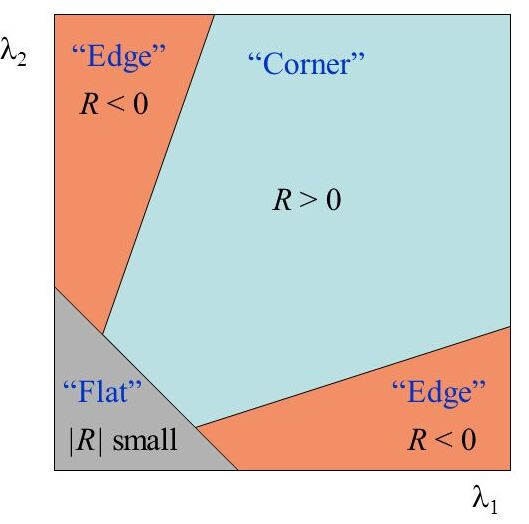
\includegraphics[width=.95\linewidth]{images/eigenvalues.jpg}    
\end{center}

\newpage 

\addcontentsline{toc}{section}{Harris Corner Detector - Algorithm}
\section*{Harris Corner Detector - Algorithm}

The Harris Corner Detector algorithm consists of the following steps:

\begin{enumerate}[start=0]
    \item \textbf{Preprocessing}: convert the original image into a grayscale image $I$. The pixel values of $I$ are computed as a weighted sum of the corresponding $R, G, B$ values:
    \begin{equation*}
        I = 0.299R + 0.587G + 0.114B
    \end{equation*}
    \item \textbf{Compute the derivatives $I_x$ and $I_y$} by convolving the image $I$ with a first derivative kernel, like the Sobel operator:

    \begin{center}
    $I_x = 
    \begin{bmatrix}
    +1 & 0 & -1 \\
    +2 & 0 & -2 \\
    +1 & 0 & -1 \\
    \end{bmatrix} * I$

    $I_y = 
    \begin{bmatrix}
    +1 & +2 & +1 \\
    0 & 0 & 0 \\
    -1 & -2 & -1 \\
    \end{bmatrix} * I$
    \end{center}

    Another way is to convolve with the derivative of the Gaussian to have better results.
    
    \item \textbf{[Optional] Subtract the mean from each image gradient} to eliminate the influence of the global intensity changes in the image.
    
    \item \textbf{Compute the products of the derivatives} $I_xI_x, I_xI_y, I_yI_y$;

    \item \textbf{Compute the sums of the products of derivatives} at each pixel: the next step is to sum the previously computed products over a small window around each pixel. This is done to obtain a measure of the local structure of the image. We obtain $S_{x^2}(x,y)$, $S_{xy}(x,y) = S_{xy}(x,y) $ and $ S_{y^2}(x,y)$.

    \item \textbf{Define the structure tensor (second moment matrix)} in that pixel:

    \begin{equation*}
    M(x,y) = 
    \begin{bmatrix}
    S_{x^2}(x,y) & S_{xy}(x,y) \\
    S_{xy}(x,y) & S_{y^2}(x,y)
    \end{bmatrix}
    \end{equation*}
    
    \item Compute the Harris response in that pixel:
    \begin{equation*}
        R = det(M) - k\ tr(M)^2 = \lambda_1 \lambda_2 - k\ (\lambda_1 + \lambda_2)^2
    \end{equation*}
    
    \item Compute eigenvectors and eigenvalues;
    
    \item Use threshold on eigenvalues to detect corners;

\end{enumerate}

\newpage

\addcontentsline{toc}{section}{Eigenvalues and Eigenvectors computation}
\section*{Eigenvalues and Eigenvectors computation}

The eigenvectors of a matrix $M$ are the vectors $e$ that satisfy:

\begin{equation*}
    M\ e = \lambda\ e
\end{equation*}

\begin{equation*}
    (M - \lambda I)e = 0
\end{equation*}

\begin{itemize}
    \item \textbf{$e$} $\rightarrow$ eigenvector
    \item \textbf{$\lambda$} $\rightarrow$ eigenvalue corresponding to eigenvector $e$
\end{itemize}

The steps to compute eigenvectors and eigenvalues of a matrix $M$ are the following:

\begin{itemize}
    \item Compute the determinant of $M - \lambda I$. This returns the \textbf{characteristic polynomial} of the matrix;
    \item Find the roots of the characteristic polynomial: $det(M - \lambda I) = 0$. This returns the eigenvalues;
    \item For each eigenvalue, solve: $(M - \lambda I)e=0$. This returns the eigenvectors.
\end{itemize}

Once you have the eigenvectors and the eigenvalues of a matrix $M$, you can rewrite $M$ in the following way:

\begin{equation*}
    M = \begin{bmatrix} 
        u_1 & u_2 & ... & u_d 
    \end{bmatrix} 
    M 
    \begin{bmatrix} 
        u_1 \\ u_2 \\ ... \\ u_d 
    \end{bmatrix} 
\end{equation*}

being $M$ of size $d \times d$.

\addcontentsline{toc}{section}{Trace of a matrix}
\section*{Trace of a matrix}

The trace of a $d\times d$ matrix $M$ is the sum of all the elements in its diagonal:

\begin{equation*}
    tr(M) = \sum_{i}^{d} a_{ii} = a_{1,1} + a_{2,2} + ... + a_{d,d}
\end{equation*}

\newpage

\addcontentsline{toc}{section}{Other Response Functions}
\section*{Other Response Functions}

We can use other response functions: \\

Harris $\&$ Stephens (1988):
\begin{equation*}
    R = det(M) - k\ tr(M)^2 = \lambda_1 \lambda_2 - k\ (\lambda_1 + \lambda_2)^2
\end{equation*}

Kanade $\&$ Tomasi (1994):
\begin{equation*}
    R = min(\lambda_1, \lambda_2)
\end{equation*}

Nobel (1998):
\begin{equation*}
    R = \frac{det(M)}{tr(M) + \epsilon}
\end{equation*}

\newpage

\addcontentsline{toc}{section}{Harris Corner Detector - Properties}
\section*{Harris Corner Detector - Properties}

We want to always find the same point on an object, regardless of changes in the image. To do so, the Corner detector should be insensitive to:

\begin{itemize}
    \item scale;
    \item rotation;
    \item lighting;
    \item perspective imaging;
    \item partial occlusion;
\end{itemize}

The Harris Corner Detector is:
\begin{itemize}
    \item \textbf{invariant to rotation}: the ellipse rotates but its shape given by the eigenvalues remains the same; corner response $R$ is invariant to image rotation;
    \item \textbf{invariant to intensity changes} in the image: 
    \begin{itemize}
        \item invariance to intensity shift: shifting the intensity values of the image uniformly does not affect the gradients of the image. The Harris Corner Detector operates on the gradients of the image, so any constant shift in the intensity values will be cancelled out when computing the gradients. Therefore, the Harris Corner Detector will produce the same results regardless of any uniform shift in the image intensity values;
        \item not fully invariant to intensity scale: because of the fixed intensity threshold we have only partial invariance on multiplicative intensity changes: it can detect false positives;
    \end{itemize}
\end{itemize}

\textbf{Harris Corner Detector is not invariant to scale}. \\

In edge detection, the goal is to identify boundaries or transitions between regions of the image that have different pixel values or intensities. This is typically achieved by computing the gradient of the image, which represents the rate of change in pixel values or intensities in different directions. However, the gradient operator used in edge detection is typically based on a fixed kernel size or filter, such as the Sobel or Canny operators. This means that \textbf{the operator is tuned to detect edges at a specific scale or size of features in the image}. If the feature in the image are larger or smaller than the scale the operator is tuned to, the resulting edge or corner detection may not be accentuate or may miss important features. \\

\newpage

\addcontentsline{toc}{section}{Blobs}
\section*{Blobs}

A blob can be defined as am amorphous group of connected pixels that share common properties, such as color or intensity. Blob detection algorithms aim to isolate and extract these regions from an image. Blob detection has several advantages:

\begin{itemize}
    \item \textbf{Scale-invariant detection}: Blobs are detected at multiple scales. This allows us to identify blobs that may have different sizes or shapes in the image. In contrast, corner detection typically only works at a single scale and may miss features that are smaller or larger than the scale it is tuned to.
    \item \textbf{Robustness to noise}: Blob detection is often more robust to noise and variations in lighting conditions than corner detection. This is because blobs are typically larger regions of the image and can be more easily distinguished from the background noise. In contrast, corner detection is more sensitive to noise and may produce false positives or miss something in noisy images.
\end{itemize}

\addcontentsline{toc}{section}{Scale Invariant Detection (Blob Detection)}
\section*{Scale Invariant Detection (Blob Detection)}

We want to build a detection method that will identify features that are invariant to changes in orientation, illumination and \textbf{scale}, such as \textbf{blobs}. We talk about \textbf{blob detection}. \\ 

\textbf{Methods such as blob detection are scale invariant because they detect features at multiple scales}.\\

Intuitively, we can define a function $f$ on a region that is scale invariant, i.e. that results in the same output if applied on a certain region even at different scales (for example, average intensity function is the same for corresponding regions, even at different sizes). Then we could simply take a local maximum of this function on different scales of the image. A good function will have one stable sharp peak in the key point. \\

Instead of computing $f$ for larger and larger windows, we can implement an algorithm that will use a fixed size window over a \textbf{scale space}. The scale space refers to a series of images generated by applying Gaussian blurring to the original image at different scales. It is used to analyze the image at multiple levels of detail, allowing the detection of blobs at various sizes.\\ 

Blob detection algorithms often analyze the scale space by computing the difference of Gaussians (DoG) or Laplacian of Gaussian (LoG) images. The DoG image is obtained by subtracting two adjacent scales in the scale space, while the LoG image is generated by convolving the scale space with the Laplacian operator. These operations help identify regions with significant intensity changes across scales, which are indicative of potential blobs. \\

\begin{comment}

In the scale space representation, each level or scale corresponds to a different standard deviation (sigma) value for the Gaussian kernel. The sigma determines the size of the kernel. Generally, larger sigma values result in larger kernel sizes, while smaller sigma values correspond to smaller kernel sizes.

When constructing the scale space, the process typically starts with an initial scale (sigma) and the corresponding Gaussian kernel size. The subsequent scales are then generated by progressively increasing or decreasing the sigma value and adjusting the kernel size accordingly.

The choice of scale increments or decrements depends on the specific implementation or algorithm. In some cases, a constant ratio, such as a doubling or halving of the sigma value, may be used. This ensures a logarithmic scale space, allowing for a more uniform sampling of the image's frequency content.
\end{comment}

\addcontentsline{toc}{section}{Scale space}
\section*{Scale space}

The first step is to build the scale space. The scale space refers to a series of images generated by applying Gaussian blurring to the original image at different scales. It is used to analyze the image at multiple levels of detail, allowing the detection of blobs at various sizes.

\begin{itemize}
    \item \textbf{Define a range of scales}: determine the range of scales that identifies the desired range of blob sizes we want to detect;
    \item \textbf{Generate a Gaussian kernel for each scale}: for each scale compute the Gaussian function with the sigma value of the scale and discretize it into a matrix of appropriate dimensions. The size of the matrix (kernel) can be established using sigma.
    \item \textbf{Convolve the image with each Gaussian kernel}: convolve the original image with each Gaussian kernel to obtain a series of blurred images; store each of them in the scale space.
\end{itemize}

Once the scale space is constructed, it can be further analyzed using techniques like the difference of Gaussians (DoG) or Laplacian of Gaussian (LoG) to detect and localize blobs at different scales.

\newpage

\addcontentsline{toc}{section}{Laplacian of Gaussian (LoG)}
\section*{Laplacian of Gaussian (LoG)}

A common definition for $f$ is the \textbf{Laplacian of Gaussian (LoG)}, that is the second derivative of the Gaussian filter.

\begin{center}
    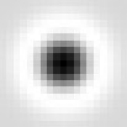
\includegraphics[width=.3\linewidth]{images/laplacian_of_gaussian.jpg}    
\end{center}

\begin{equation*}
    \nabla^2g = \frac{\delta^2g}{\delta x^2} + \frac{\delta^2g}{\delta y^2} 
\end{equation*}

When applying a scale-invariant filter like the Laplacian of Gaussian (LoG) to an image, \textbf{the maximum response is typically obtained at the scale that best matches the size of the feature being detected} (the zero of the Laplacian has to be aligned with the blob). \\

For example, if the feature being detected is a small point, the maximum response will be obtained at a small scale (i.e., a small value of the filter scale parameter). If the feature being detected is a larger object, the maximum response will be obtained at a larger scale (i.e., a larger value of the filter scale parameter). \\

\begin{center}
    \begin{tabular}{llllll}
        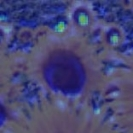
\includegraphics[width=.14\linewidth]{images/scale_0.jpg} &
        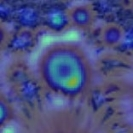
\includegraphics[width=.14\linewidth]{images/scale_1.jpg} & 
        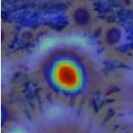
\includegraphics[width=.14\linewidth]{images/scale_2.jpg} & 
        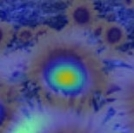
\includegraphics[width=.14\linewidth]{images/scale_3.jpg} & 
        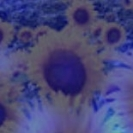
\includegraphics[width=.14\linewidth]{images/scale_4.jpg} & 
        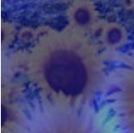
\includegraphics[width=.14\linewidth]{images/scale_5.jpg} \\
        \text{$\sigma = 2.1$} & 
        \text{$\sigma = 4.2$} &
        \text{$\sigma = 6.0$} &
        \text{$\sigma = 9.8$} &
        \text{$\sigma = 15.5$} &
        \text{$\sigma = 17.0$} \\
    \end{tabular}
\end{center}

\begin{comment}
Instead of computing $f$ for larger and larger windows, we can implement an algorithm that will use a fixed size window over a \textbf{scale space}. Only the scaling factor of the filter ($\sigma$ for a Gaussian in this case) will change across iterations. \\
\end{comment}

Here's how the LoG-based blob detection process typically proceeds within the scale space: \\

For each scale in the scale space:
\begin{itemize}
    \item Determine the standard deviation (sigma) value corresponding to the current scale;
    \item Compute the kernel size based on the relationship between kernel size and sigma. The size of the kernel is determined to capture the desired blurring effect at the current scale;
    \item Generate the LoG kernel using the calculated kernel size.
    \item Convolve the current scale image with the LoG kernel to obtain the LoG response image, which represents the Laplacian of the blurred image at that scale. This image will have some local maxima based on some threshold.
\end{itemize}

When using the Laplacian of Gaussian (LoG) for blob detection with the scale space, the kernel size does not remain the same for each image in the scale space. The kernel size varies across different scales to correspond to the appropriate blurring level.\\

Once we have all the LoG response images, each with some local maxima, for each feature compute the cross-scale maxima. Save its coordinates along with the scale $(x, y, \sigma)$ .

\addcontentsline{toc}{section}{Naive Blob Detector Implementation}
\section*{Naive Blob Detector Implementation}

Pseudocode:
\begin{minted}{python}
    for each level of the scale space:
        compute the feature response (e.g. Laplacian)

    # now, for each level (scale) we have a set of features 

    for each level of the scale space:
        if one feature is the local maximum (filter highlights blob in that feature) 
            and cross-scale maximum (maximum filter response across levels):
                save scale and location of the feature (x,y,s)
    
\end{minted}

\begin{center}
    \begin{tabular}{lll}
        \text{} &
        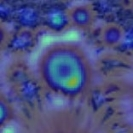
\includegraphics[width=.14\linewidth]{images/scale_1.jpg}  & 
        \text{local maximum} \\

        \text{cross-scale maximum} &
        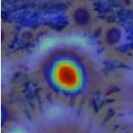
\includegraphics[width=.14\linewidth]{images/scale_2.jpg}  & 
        \text{local maximum} \\

        \text{} &
        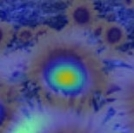
\includegraphics[width=.14\linewidth]{images/scale_3.jpg}  & 
        \text{local maximum} \\
    \end{tabular}
\end{center}

\hspace{0.5cm}

For more information about the algorithm and a python implementation, you can read \href{https://projectsflix.com/opencv/laplacian-blob-detector-using-python/}{here}.

\newpage

\addcontentsline{toc}{section}{Difference of Gaussian (DoG)}
\section*{Difference of Gaussians (DoG)}

The LoG is very similar to a Difference of Gaussians (DoG), that is a Gaussian minus a slightly smaller Gaussian:
\begin{center}
    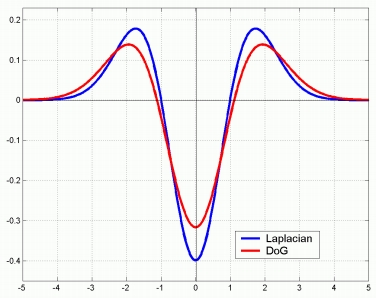
\includegraphics[width=.6\linewidth]{images/log_dog.jpg}
\end{center}

Gaussian:
\begin{equation*}
    G(x,y,\sigma) = \frac{1}{\sqrt{2\pi }\sigma}e^{-\frac{x^2+y^2}{2\sigma^2}}
\end{equation*}

Laplacian of Gaussian:
\begin{equation*}
    LoG = \nabla^2g = \frac{\delta^2g}{\delta x^2} + \frac{\delta^2g}{\delta y^2} 
\end{equation*}

Difference of Gaussians:
\begin{equation*}
    DoG = G(x,y,k\sigma) - G(x,y,\sigma)    
\end{equation*}

Since we have to use a Gaussian scale space it is very convenient to use the DoG instead of the LoG: the response function can simply be the difference from a window on one layer of the pyramid and the same window on the upper layer. More information about the DoG algorithm can be found \href{https://medium.com/@vad710/cv-for-busy-devs-improving-features-df20c3aa5887#:~:text=The%20Difference%20of%20Gaussian%20(DoG)%20technique%20is%20a%20highly%20influential,adjacent%20images%20from%20each%20other.}{here}

\begin{center}
    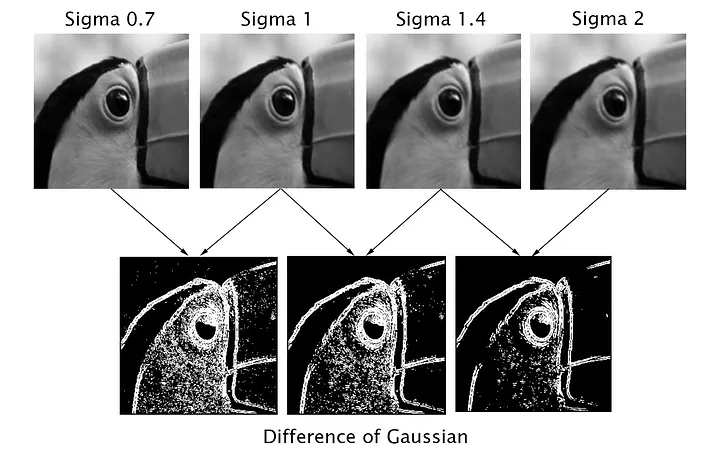
\includegraphics[width=.9\linewidth]{images/dog.png}
\end{center}

The Difference of Gaussian technique evolved from the Laplacian of Gaussian (LoG) technique. It turns out that subtracting Gaussian images from each other is a speedy estimation of the Laplacian of Gaussian. The Difference of Gaussian technique is a less compute intensive approximation of a Laplacian of Gaussian calculation.

\newpage

\addcontentsline{toc}{section}{Feature Descriptor}
\section*{Feature Descriptor}

After an object or a region of interest is detected in an image, a feature descriptor is used to represent the detected object or region in a compact and distinctive way. This is necessary because raw pixel values of an image can be noisy, redundant, and not invariant to scale, orientation, and illumination changes, which can make object recognition and matching difficult. \\

A feature descriptor is a representation of an object or a region of interest in an image that captures its unique characteristics. Feature descriptors are designed to be robust to common image transformations, such as rotation, scale, and illumination changes. They are also designed to be efficient to compute and store. \\

\textbf{Patches with similar content should have similar descriptors}.

\addcontentsline{toc}{section}{Naive Feature Descriptors}
\section*{Naive Feature Descriptors}

\begin{itemize}
    \item \textbf{image patch}: just use the plain image patch (flattened to array) to describe the feature; this is perfectly fine if geometry and appearance remain unchanged (i.e. in \textbf{template matching}, the process of moving the template over the entire image and calculating the similarity between the template and the covered window on the image); The problem with this approach is that \textbf{small changes in the intensity values of the pixels within the patch can lead to significant changes in the feature descriptor};
    \item \textbf{image gradients}: use the intensity variation instead of the intensity values; this way the feature is invariant to absolute intensity values; \textbf{How can it be less sensitive to deformations?}
    \item \textbf{color histogram}: count the colors in the image using a histogram; this is invariant to changes in scale and rotation; the problem with this approach is that \textbf{we loose spatial information}: two completely different patches with the same colors will have the same descriptor.
    \item \textbf{spatial histograms}: compute histograms over spatial cells; the descriptor divides the image into a grid of cells and then counts the number of occurrences of each visual feature in each cell. The resulting counts are organized into a histogram, where each bin corresponds to a range of values for the visual feature. This technique is partially invariant to rotation; \textbf{how can it be completely invariant to rotation?}
    \item \textbf{orientation normalization}: use the dominant image gradient direction to normalize the orientation of the patch; this is typically achieved by computing the dominant orientation of the image feature and then rotating the image patch; the problem with this approach is that orientation of an image feature can be sensitive to changes in scale, which can lead to inconsistencies in the descriptor when comparing features at different scales.
\end{itemize}

\addcontentsline{toc}{section}{Histogram of Oriented Gradients (HOG) Descriptor}
\section*{Histogram of Oriented Gradients (HOG) Descriptor}

For detailed steps and a python implementation, you can check \href{https://www.analyticsvidhya.com/blog/2019/09/feature-engineering-images-introduction-hog-feature-descriptor/}{this} out.
\href{https://www.analyticsvidhya.com/blog/2019/09/feature-engineering-images-introduction-hog-feature-descriptor/}{Here} is a great video explaination of the HOG Descriptor.

\begin{enumerate}[start=0]
    \item \textbf{preprocessing}: preprocess the image and bring down the width to height ratio to 1:2. The image size should preferably be $64\times 128$. This is because we will be dividing the image into $8\times8$ and $16\times16$ patches to extract the features. Having the specified size $64\times 128$ will make the calculations pretty simple;
    \item \textbf{image gradients}: the next step is to compute the gradients;
    \item \textbf{magnitude and orientation}: once we have the gradients, we can compute magnitude and orientation for each pixel in the $8\times 8$ patch;
    \item \textbf{generate the histogram}: generate an histogram with magnitude and orientation for each $8\times 8$ cell;
    \item \textbf{normalize the gradients}: the gradients of the image are sensitive to the overall lighting. This means that for a particular picture, some portion of the image would be very bright as compared to the other portions. We cannot completely eliminate this from the image, but we can reduce this lighting variation by normalizing the gradients by taking $16\times 16$ blocks. A $16\times 16$ block has $4$ histograms which can be concatenated to form a $36\times 1$ element vector. This vector is normalized with \textbf{L2 norm}. \\

    Given a vector $v$:
    \begin{equation*}
        v = \begin{bmatrix}
            v_1 & v_2 & ... & v_n
        \end{bmatrix}
    \end{equation*}

    Compute the L2 norm:
    \begin{equation*}
        k = \sqrt{v_1^2 + v_2^2 + ... + v_n^2}
    \end{equation*}

    Divide each component in the vector $v$ by $k$:
    \begin{equation*}
        nv = \begin{bmatrix}
            \frac{v_1}{k} & \frac{v_2}{k} & ... \frac{v_n}{k} 
        \end{bmatrix}
    \end{equation*}

    \item \textbf{shift the window}: the window is then moved by $8$ pixels and a normalized $36\times 1$ vector is calculated, the process is repeated. The feature is the centroid of the $16\times 16$ block.

\end{enumerate}

\newpage

\addcontentsline{toc}{section}{Histogram generation}
\section*{Histogram generation}

The naive way to generate the histogram is to divide the $0-180$ spectrum (unsigned) into bins (we will use $9$ bins, each spanning $20$ degrees) and to count the occurrences of the orientation. \textbf{This does not take into account the magnitude}. Instead of using the frequency, we can use the gradient magnitude to fill the values in the matrix: 

\begin{center}
    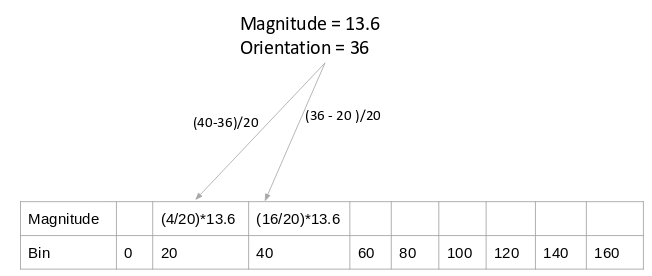
\includegraphics[width=.9\linewidth]{images/hog_histogram.png}
\end{center}

\newpage

\addcontentsline{toc}{section}{Scale invariance}
\section*{Scale invariance}

The HOG descriptor is partially invariant to scale. The HOG descriptor is based on the distribution of gradients in an image, and the gradients are computed over small image patches. \\

When the image is scaled up or down, the size of the patches also changes accordingly. However, the HOG descriptor compensates for this scale change by normalizing the histogram bins for each patch based on the overall gradient energy within that patch. This normalization helps to ensure that the descriptor is partially invariant to changes in scale. \\

However, \textbf{if the scale change is too significant, the HOG descriptor may not perform well}. For example, \textbf{if an object is very small in the image, its HOG descriptor may not be distinctive enough for reliable object recognition}. Similarly, \textbf{if an object is very large in the image, its HOG descriptor may become too coarse, resulting in loss of fine-grained details}. Therefore, it is important to carefully choose the scale of the image and the size of the patches when using the HOG descriptor for object recognition.

\addcontentsline{toc}{section}{Scale Invariant Feature Transform (SIFT)}
\section*{Scale Invariant Feature Transform (SIFT)}

Scale Invariant Feature Transform (SIFT) \textbf{consist of both a detector and a descriptor}. \\

Feature detector:
\begin{itemize}
    \item \textbf{Multi-scale extrema (keypoint) detection};
    \item \textbf{Keypoint localization};
    \item \textbf{Orientation assignment};
\end{itemize}

Feature descriptor:
\begin{itemize}
    \item \textbf{Keypoint descriptor};
\end{itemize}

The idea is that proper scaling of objects in new image is unknown; exploring features in different scales is helpful to recognize different objects.\\

For more information about the SIFT algorithm you can read \href{https://medium.com/data-breach/introduction-to-sift-scale-invariant-feature-transform-65d7f3a72d40/}{here}.

\newpage

\addcontentsline{toc}{section}{SIFT Detector - keypoint detection}
\section*{SIFT Detector - Keypoint detection}

The first step of the SIFT algorithm is to detect keypoints in an image. Keypoints are distinctive features in an image that can be used to identify the same object in different images. \\

An octave is a set of images of the same size blurred at different scales. Each octave's image size is half the previous one. 

\begin{center}
    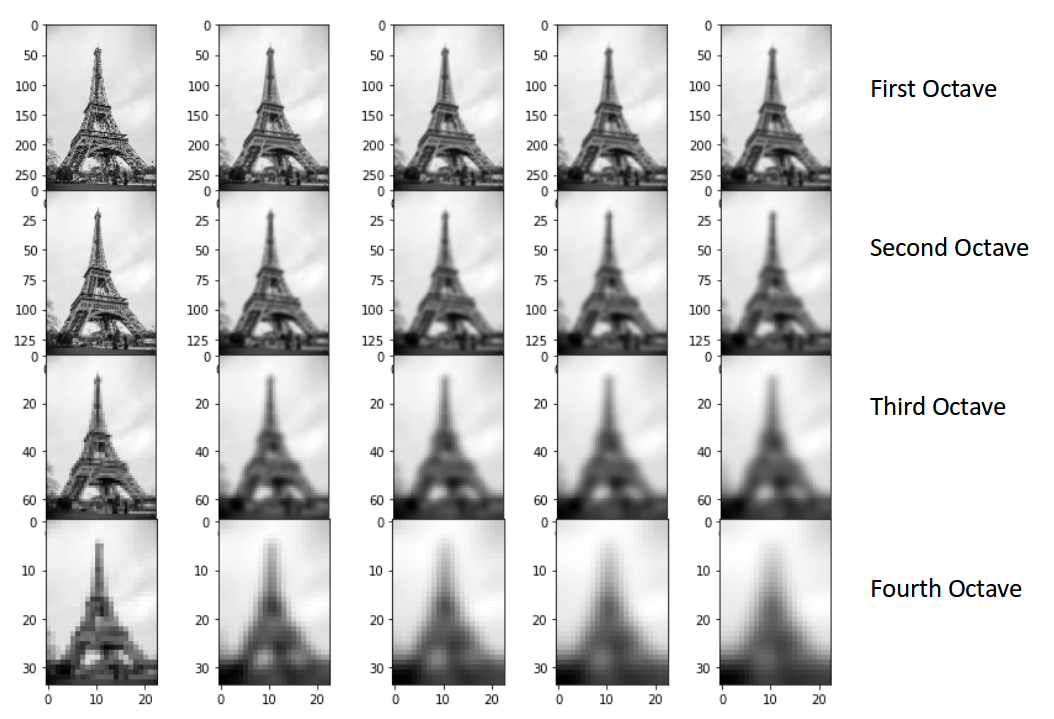
\includegraphics[width=.9\linewidth]{images/octaves.png}
\end{center}

Now we use those blurred images to generate another set of images, the Difference of Gaussians (DoG). These DoG images are great for finding out interesting keypoints in the image. The difference of Gaussian is obtained as the difference of Gaussian blurring of an image with two different $\sigma$, let it be $\sigma$ and $k\sigma$. This process is done for different downsampling layers. This is what the process looks like:

\begin{center}
    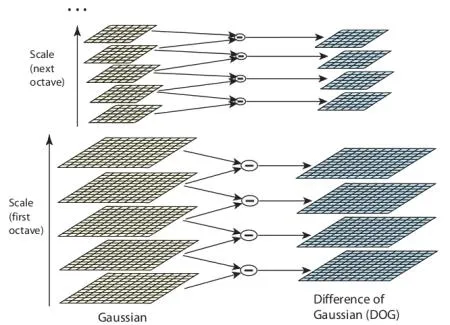
\includegraphics[width=.6\linewidth]{images/octave_dog.png}
\end{center}

\addcontentsline{toc}{section}{SIFT Detector - keypoint localization}
\section*{SIFT Detector - Keypoint localization}

We have generated a scale space and used the scale space to calculate the Difference of Gaussians. Those are used to approximate Laplacian of Gaussian (LoG).

\begin{center}
    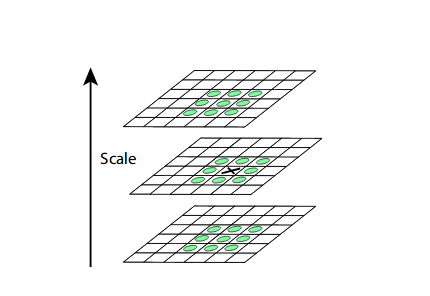
\includegraphics[width=.6\linewidth]{images/sift_keypoint_localization.png}
\end{center}

One pixel in an image is compared with its 8 neighbors as well as 9 pixels in the next scale and 9 pixels in previous scales. This way, a total of 26 checks are made. If it is a local extrema, it is a potential keypoint. It basically means that keypoint is best represented in that scale (the scale of the considered blurred image in the DoG set $\sigma$). The keypoint is thus identified by $\textbf{x} = \{x, y, \sigma\}$.

\addcontentsline{toc}{section}{SIFT Detector - keypoint localization - keypoint stability}
\section*{SIFT Detector - Keypoint localization - Keypoint stability}

The previous step produces a lot of keypoints. Some of them lie along an edge, or they don’t have enough contrast. In both cases, they are not as useful as features, so we get rid of them. \\

Removing low contrast features: if the magnitude of the intensity of the blurred image at the current pixel in the DoG is less than a certain value, then the pixel is rejected (typically a pixel with a magnitude intensity that is less than $0.1$ the max value). This is done because low contrast is generally less reliable than high contrast for feature points. 

\newpage

\addcontentsline{toc}{section}{SIFT Detector - Orientation assignment}
\section*{SIFT Detector - Orientation assignment}

The next step consists in assigning an orientation to each keypoint; this provides rotation invariance. \\

For all the levels:
\begin{itemize}
    \item \textbf{compute the magnitude and orientation}: a neighborhood is taken around the keypoint location (its size depends on the scale of the level), and the gradient magnitude and direction is calculated in that region;
    \item \textbf{compute the weighted magnitude + orientation histogram}: an oriented histogram with $36$ bins covering $360$ degrees is created; the amount of the orientation added to a certain bin is proportional to the magnitude of the gradient at that point;
    \item \textbf{find the peak of the histogram}: the bin of the highest peak is used for the orientation of the keypoint. \\
    
    Furthermore, any peaks above 80\% of the highest peak are converted into a new keypoint; This new keypoint has the same location and scale as the original, but its orientation is different.
\end{itemize}

\addcontentsline{toc}{section}{SIFT Descriptor - keypoint description}
\section*{SIFT Descriptor - Keypoint description}

At this point, each keypoint has a location, scale, orientation. Next is to compute a descriptor for the local image region about each keypoint that is highly distinctive and invariant as possible to variations such as changes in viewpoint and illumination. \\

The steps of building the SIFT descriptor are as following:

\begin{itemize}
    \item use the \textbf{Gaussian blurred image} associated with the keypoint's scale;
    \item take \textbf{image gradients over a $16\times16$ square window} around the detected feature;
    \item \textbf{rotate the gradient} directions AND locations relative to the keypoint orientation (given by the dominant orientation);
    \item \textbf{divide the 16x16 window into a $4\times4$ grid of cells};
    \item \textbf{compute an orientation histogram} with $8$ orientations bins for each cell bins (summing the weighted gradient magnitude);
    \item the \textbf{resulting SIFT descriptor is a length $128$ vector} representing a $4\time4$ histogram array with $8$ orientation bins per histogram;
\end{itemize}

\newpage

\addcontentsline{toc}{section}{SIFT Descriptor Properties}
\section*{SIFT Descriptor Properties}

\begin{itemize}
    \item \textbf{invariant to rotation} because we rotated the gradients; we are assuming the rotated image will generate a key point at the same location as the original image;
    \item \textbf{invariant to scale} because we worked with the scaled image from DoG;
    \item \textbf{invariant/robustness to illumination variation} since we worked with the orientation and we don’t take in consideration the magnitude of the gradient (alone);
    \item \textbf{slight robustness to affine transformation and to noise} (empirically found);
\end{itemize}

\newpage

\addcontentsline{toc}{section}{Keypoint matching}
\section*{Keypoint matching}

Keypoint matching is a technique used in computer vision to identify and match the corresponding keypoints in multiple images. The process involves identifying keypoints in multiple images and then finding the corresponding keypoints between them. 

\begin{itemize}
    \item \textbf{Find all keypoints} in a target image. Each keypoint will have 2D location, scale and orientation, as well as invariant descriptor vector (x,y,s,theta,d). This can be done using various algorithms such as SIFT, SURF, ORB, and AKAZE.
    \item \textbf{For each keypoint, search similar descriptor vectors} in the other image(s).
    \item Once the keypoints are matched, \textbf{they can be used to compute the transformation between the two images}. 
\end{itemize}

One problem is that \textbf{the descriptor vector may match more than one reference in the database}.

\addcontentsline{toc}{section}{Feature matching}
\section*{Feature matching}

\textbf{Given a feature in $I_1$, how to find the best match in $I_2$?}

\begin{enumerate}
    \item Define distance function that compares two descriptors;
    \begin{itemize}
        \item Simple approach: $L2$ norm.
        \begin{equation*}
            d = |f_1 - f_2|
        \end{equation*}
        Can give small distances for ambiguous (incorrect) matches;
        \item Better approach: distance ratio.
        \begin{equation*}
            d = \frac{|f_1 - f_2|}{|f_1 - f_2'|}
        \end{equation*}
        \begin{center}
            \textit{$f_2$ is the best match to $f_1$ in $I_2$} \\
            \textit{$f_2'$ is the second best match to $f_1$ in $I_2$}
        \end{center}
        To further improve this method we can \textbf{set the distance ratio threshold ($\rho$) to around $0.5$}, which means that we require our best match to be at least twice as close as our second best match to our initial features descriptor. 
    \end{itemize}
    \item Test all the features in $I_2$, find the one that minimizes the distance function;
\end{enumerate}

\newpage

\addcontentsline{toc}{section}{Invariance properties}
\section*{Invariance properties}

\begin{itemize}
    \item \textbf{Canny edge detector}:
    \begin{itemize} 
        \item \textbf{Rotation Invariant}: Both yes and no. Will an edge that is detected in the original image also be detected after rotating the image? Theorically yes, but the output edges will change.
        \item \textbf{Scale Invariant}: No, the Canny edge detector is not scale invariant. The detected edges may vary if the image is scaled.
        \item \textbf{Intensity Shift Invariant}: Yes, the Canny edge detector is intensity shift invariant. It detects edges based on intensity gradients, so shifting the overall intensity does not affect the results.
        \item \textbf{Intensity Scale Invariant}: Yes, the Canny edge detector is intensity scale invariant. It calculates gradients and applies a threshold, which is relative to the image's intensity. Scaling the intensity uniformly across the image will not affect the edge detection.
    \end{itemize}

    \item \textbf{Harris corner detector}:
    \begin{itemize}
        \item \textbf{Rotation Invariant}: Yes, the Harris corner detector is rotation invariant. The detected corners will not change if the image is rotated.
        \item \textbf{Scale Invariant}: No, the Harris corner detector is not scale invariant. The detected corners may vary if the image is scaled.
        \item \textbf{Intensity Shift Invariant}: Yes, the Harris corner detector is intensity shift invariant. It detects croenrs based on intensity gradients, so shifting the overall intensity does not affect the results (only derivatives are used, $I \rightarrow I + b$).
        \item \textbf{Intensity Scale Invariant}: Partially, because of the fixed threshold on local maxima. Yes if the threshold is relative to the image's intensity. Scaling the intensity uniformly across the image will not affect the edge detection if we account for it with the thresold.
    \end{itemize}

    \item \textbf{LoG (Laplacian of Gaussian) blob detector}:
    \begin{itemize}
        \item \textbf{Rotation Invariant}: Yes, the LoG blob detector is rotation invariant. It convolves the image with a Laplacian of Gaussian filter, which is rotationally symmetric.
        \item \textbf{Scale Invariant}: Yes, the LoG blob detector is scale invariant. The Laplacian of Gaussian operator is applied at multiple scales to detect blobs of different sizes.
        \item \textbf{Intensity Shift Invariant}: Yes, the LoG blob detector is intensity shift invariant. It calculates responses based on the second derivative of intensity, so shifting the overall intensity does not affect the results.
        \item \textbf{Intensity Scale Invariant}: Yes, the LoG blob detector is intensity scale invariant. The Laplacian of Gaussian operator applies a scale-normalized filter, so scaling the intensity uniformly across the image will not affect the blob detection.
    \end{itemize}

    \item \textbf{SIFT (Scale-Invariant Feature Transform)}:
    \begin{itemize}
        \item \textbf{Rotation Invariant}: Yes, SIFT is rotation invariant. It uses orientation histograms to compute features that are invariant to image rotation.
        \item \textbf{Scale Invariant}: Yes, SIFT is scale invariant. It applies scale-space extrema detection to detect features at different scales.
        \item \textbf{Intensity Shift Invariant}: Yes, SIFT is intensity shift invariant. It uses normalized gradient magnitudes to calculate feature descriptors, which are invariant to intensity shifts.
        \item \textbf{Intensity Scale Invariant}: Yes, SIFT is intensity scale invariant. It uses a scale-normalized Gaussian kernel in the construction of the scale-space pyramid, making it invariant to intensity scaling.
    \end{itemize}

\end{itemize}

\newpage

\addcontentsline{toc}{section}{Homografy}
\section*{Homografy}

Homography refers to a mathematical transformation that relates the coordinates of points on a plane to the coordinates of those same points when viewed from a different perspective or angle. \\

In computer vision and image processing, homography is commonly used to correct distortions caused by perspective projection, such as those that occur when viewing a three-dimensional object from different angles or when taking photographs with a camera that is not aligned perfectly with the scene being photographed. \\

A homography can be represented by a $3\times3$ matrix and is typically computed by finding correspondences between points in two different images or frames. Once a homography has been computed, it can be used to warp or transform one image to match the perspective of the other image, or to estimate the pose or position of a camera relative to a scene.

\newpage

\addcontentsline{toc}{section}{RAndom SAmple Consensus (RANSAC)}
\section*{RAndom SAmple Consensus (RANSAC)}

RANSAC, which stands for \textbf{RAndom SAmple Consensus}, is a robust algorithm commonly used in computer vision and machine learning to estimate parameters of a mathematical model from a set of observed data that contains outliers or noise. \\

The basic idea behind RANSAC is to randomly sample a subset of the data, fit a model to the sample, and then use the model to classify the remaining data as inliers or outliers. This process is repeated multiple times, and the model with the largest number of inliers is selected as the final estimate of the parameters. \\

\textbf{RANSAC can be applied to a wide range of problems, such as estimating the parameters of a homography}, detecting and removing outliers in data, or fitting a line or curve to a set of noisy points. \\

One of the key advantages of RANSAC is its ability to handle outliers and noise in the data, which can cause traditional methods to fail or produce unreliable results. However, \textbf{RANSAC does have some limitations}, such as the need to choose appropriate parameters for the algorithm, and the potential for the algorithm to get stuck in local optima or to converge to suboptimal solutions.\\

The main steps are the following:
\begin{itemize}
    \item randomly choose s samples; Typically s is the minimum sample size that lets you fit a model;
    \item fit a model (e.g. line) to those samples;
    \item count the number of inliers that approximately fit the model;
    \item repeat n times;
    \item choose the model that has the largest set of inliers;
\end{itemize}

\textbf{Each hypothesis gets voted on by each data point; the best hypothesis wins.}

\newpage

\addcontentsline{toc}{section}{Image alignment and Image stitching}
\section*{Image alignment and Image stitching}

Image alignment and image stitching are two related concepts in computer vision that are used to combine multiple images into a larger panorama or composite image. While they are often used together, they refer to different aspects of the image processing pipeline.

\addcontentsline{toc}{section}{Image alignment}
\section*{Image alignment}

\textbf{Image alignment refers to the process of aligning two or more images so that their content overlaps as closely as possible.} This is typically necessary because images that are taken from different viewpoints or at different times may have different orientations, scales, and perspectives.

Image alignment techniques typically involve:
\begin{itemize}
    \item \textbf{Compute image features for image A and image B};
    \item \textbf{Match features between A and B};
    \item \textbf{Compute a transformation that maps one image to the other (homography)}; this can be done using \textbf{RANSAC};
\end{itemize}

\addcontentsline{toc}{section}{Image stitching}
\section*{Image stitching}

\textbf{Image stitching refers to the process of combining multiple aligned images into a single composite image}. This typically involves blending the overlapping regions of the images together to create a seamless transition, and possibly correcting for distortions and artifacts that may arise during the alignment and blending process. Image stitching is often used in panoramic photography, where a series of images taken from a single viewpoint are stitched together to create a wide-angle view of a scene.

\newpage

\addcontentsline{toc}{section}{Transformations}
\section*{Transformations}

A transformation refers to the process of modifying the appearance or geometry of an image to achieve a desired effect. \textbf{A transformation $T$ is a coordinate-changing machine}.

There are various types of transformations that can be applied to images, including geometric transformations such as scaling, rotation, translation, and perspective transformation, as well as non-geometric transformations such as brightness adjustment, contrast adjustment, color space conversion, and filtering.

\begin{itemize}
    \item \textbf{Geometric transformations involve modifying the shape or position of an image or its parts}. For example, rotation can be used to change the orientation of an image, scaling can be used to change its size, and translation can be used to shift its position. Perspective transformation can be used to correct for distortion due to camera angle or lens distortion.
\end{itemize}

\begin{itemize}
    \item \textbf{Non-geometric transformations modify the visual appearance of an image without changing its shape or position}. For example, brightness and contrast adjustment can be used to enhance the visibility of an image, while color space conversion can be used to change the color representation of an image. Filtering operations can be used to smooth or sharpen an image or to remove noise or other artifacts.
\end{itemize}

A geometric transformation can be global or non-global:
\begin{itemize}
    \item A \textbf{global transformation} is the same for any point of the image;
    \item A \textbf{non-global transformation} is instead applied locally to specific regions or parts of an image;
\end{itemize}

\textbf{Let's focus on global transformations}. A global transformation can be:
\begin{itemize}
    \item \textbf{linear} if it can be described by a $2\times 2$ matrix;
    \begin{equation*}
        p' = Tp
    \end{equation*}
    \begin{equation*}
        \begin{bmatrix}
            x' \\ y'
        \end{bmatrix}
        = T \begin{bmatrix}
            x \\ y
        \end{bmatrix}
    \end{equation*}
    \item \textbf{non-linear}
\end{itemize}

\newpage

\addcontentsline{toc}{section}{Linear transformations}
\section*{Linear transformations}

Common linear transformations include:
\begin{itemize}
    \item \textbf{Uniform scaling}:
    \begin{equation*}
        S = \begin{bmatrix}
            s & 0 \\ 
            0 & s
        \end{bmatrix}
    \end{equation*}
    \item \textbf{Rotation by angle $\theta$}:
    \begin{equation*}
        R = \begin{bmatrix}
            cos\theta & -sin\theta \\ 
            sin\theta & cos\theta
        \end{bmatrix}
    \end{equation*}
    The inverse of which is $R^{-1} = R^T$
    \item \textbf{Mirror about y axis}:
    \begin{equation*}
        T = \begin{bmatrix}
            -1 & 0 \\
            0 & 1
        \end{bmatrix}
    \end{equation*}
    \item \textbf{Mirror about x axis}:
    \begin{equation*}
        T = \begin{bmatrix}
            0 & 1 \\
            1 & 0
        \end{bmatrix}
    \end{equation*}
\end{itemize}

\textbf{Translation is not a linear transformation} on 2D coordinates.

\addcontentsline{toc}{section}{Affine transformations}
\section*{Affine transformations}

Any transformation represented by a $3\times 3$ matrix which has $\begin{bmatrix}
    0 & 0 & 1
\end{bmatrix}$
as last row, is called an \textbf{affine transformation}. We can express the previous transformations in terms of $3\times 3$ matrices, as well as translation.\\ 

\begin{equation*}
    \begin{matrix}
        \begin{bmatrix}
            x' \\ y' \\ 1
        \end{bmatrix} = 
        \begin{bmatrix}
            1 & 0 & t_x \\
            0 & 1 & t_y \\
            0 & 0 & 1
        \end{bmatrix}
        \begin{bmatrix}
            x \\ y \\ 1
        \end{bmatrix} & & 
        \begin{bmatrix}
            x' \\ y' \\ 1
        \end{bmatrix} = 
        \begin{bmatrix}
            s_x & 0 & 0 \\
            0 & s_y & 0 \\
            0 & 0 & 1
        \end{bmatrix}
        \begin{bmatrix}
            x \\ y \\ 1
        \end{bmatrix} \\
        \\
        Translate & & Scale \\
        \\
        \\
        \begin{bmatrix}
            x' \\ y' \\ 1
        \end{bmatrix} = 
        \begin{bmatrix}
            cos\theta & -sin\theta & 0 \\
            sin\theta & cos\theta & 0 \\
            0 & 0 & 1
        \end{bmatrix}
        \begin{bmatrix}
            x \\ y \\ 1
        \end{bmatrix} & & 
        \begin{bmatrix}
            x' \\ y' \\ 1
        \end{bmatrix} = 
        \begin{bmatrix}
            1 & sh_x & 0 \\
            sh_y & 1 & 0 \\
            0 & 0 & 1
        \end{bmatrix}
        \begin{bmatrix}
            x \\ y \\ 1
        \end{bmatrix} \\
        \\
        Rotate & & Shear/Deform
    \end{matrix}
\end{equation*}

\newpage

Affine transformations can be sees as:
\begin{equation*}
    \begin{bmatrix}
        x' \\ y' \\ w'
    \end{bmatrix} = 
    \begin{bmatrix}
        a & b & c \\
        d & e & f \\
        0 & 0 & 1
    \end{bmatrix}
    \begin{bmatrix}
        x \\ y \\ w
    \end{bmatrix}
\end{equation*}

Homografies/Planar Perspective Maps/Projective transformations can be sees as:
\begin{equation*}
    \begin{bmatrix}
        x' \\ y' \\ w'
    \end{bmatrix} = 
    \begin{bmatrix}
        a & b & c \\
        d & e & f \\
        g & h & 1
    \end{bmatrix}
    \begin{bmatrix}
        x \\ y \\ w
    \end{bmatrix}
\end{equation*}

\newpage

\begin{comment}

\section*{Camera calibration}

A point can be expressed with several coordinate systems:

\begin{itemize}
    \item \textbf{World coordinates}:
    \begin{equation*}
        \boldsymbol{x_w} = (x_w, y_w, z_w)^T
    \end{equation*}
    \item \textbf{Camera coordinates}:
    \begin{equation*}
        \boldsymbol{x_c} = (x_c, y_c, z_c)^T
    \end{equation*}
    \item \textbf{Image coordinate}:
    \begin{equation*}
         \boldsymbol{x_i} = (x, y) ^ T
    \end{equation*}
\end{itemize}

A $3\times 4$ \textbf{projection matrix P} denotes the relationship between $x_w$ and $x_i$:

\begin{equation*}
    \boldsymbol{x_i} = P\boldsymbol{x_w}
\end{equation*}

\begin{equation*}
    s\begin{bmatrix}
        x \\ y \\ 1
    \end{bmatrix} = \begin{bmatrix}
        p_{1, 1} & p_{1, 2} & p_{1, 3} & 
        p_{1, 4} \\
        p_{2, 1} & p_{2, 2} & p_{2, 3} & 
        p_{2, 4} \\
        p_{3, 1} & p_{3, 2} & p_{3, 3} & 
        p_{3, 4} \\
    \end{bmatrix}
    \begin{bmatrix}
        x_w \\ y_w \\ z_w \\ 1
    \end{bmatrix}
\end{equation*}

The projection matrix can be decomposed into two components: intrinsic and extrinsic parameter matrix.

\begin{equation*}
    \boldsymbol{x_i} = P\boldsymbol{x_w} = A[R|t]\boldsymbol{x_w}
\end{equation*}

\begin{equation*}
    \begin{bmatrix}
        x \\ y \\ 1
    \end{bmatrix} = 
    \begin{bmatrix}
        \alpha_x & s & x_0 \\
        0 & \alpha_y & y_0 \\
        0 & 0 & 1 \\
    \end{bmatrix}
    \begin{bmatrix}
        r_{1, 1} & r_{1, 2} & r_{1, 3} & 
        t_1 \\
        r_{2, 1} & r_{2, 2} & r_{2, 3} & 
        t_2 \\
        r_{3, 1} & r_{3, 2} & r_{3, 3} & 
        t_3 \\
    \end{bmatrix}
    \begin{bmatrix}
        x_w \\ y_w \\ z_w \\ 1
    \end{bmatrix}
\end{equation*}

\begin{itemize}
    \item the $3\times 3$ calibration matrix \textbf{A} contains the \textbf{intrinsic parameters};
    \item the $3\times 3$ rotation matrix \textbf{R} and the $3\times 1$ translation vector \textbf{t} contains the \textbf{extrinsic parameters}; 
\end{itemize}

Read \href{https://www.analyticsvidhya.com/blog/2021/10/a-comprehensive-guide-for-camera-calibration-in-computer-vision/}{here}.

\newpage

\section*{Steps to project a 2D world point to a 2D image point}

\begin{itemize}
    \item \textbf{3D world point to a 3D camera point}:
    \begin{equation*}
        \begin{bmatrix}
            x_c \\ y_c \\ z_c \\ 1
        \end{bmatrix} = 
        \begin{bmatrix}
            r_{1, 1} & r_{1, 2} & r_{1, 3} & 
            t_1 \\
            r_{2, 1} & r_{2, 2} & r_{2, 3} & 
            t_2 \\
            r_{3, 1} & r_{3, 2} & r_{3, 3} & 
            t_3 \\
        \end{bmatrix}
        \begin{bmatrix}
            x_w \\ y_w \\ z_w \\ 1
        \end{bmatrix}
    \end{equation*}
    \item \textbf{3D camera point to 2D camera point}:
    \begin{equation*}
        \begin{bmatrix}
            x_c^d \\ y_c^d \\ 1
        \end{bmatrix} = 
        \begin{bmatrix}
            f & 0 & 0 & 0 \\
            0 & f & 0 & 0 \\
            0 & 0 & 1 & 0
        \end{bmatrix}
        \begin{bmatrix}
            x_c \\ y_c \\ z_c \\ 1
        \end{bmatrix}
    \end{equation*}
        
    \begin{center}
        \textit{$f$ denotes the focal length in metric system}
    \end{center}

    \begingroup
    \Large
    \begin{equation*}
        \begin{matrix}
            x_c = \frac{f}{z_w}x_w & & y_c = \frac{f}{z_w}y_w
        \end{matrix}
    \end{equation*}
    \endgroup

    \item \textbf{Account for lens distortion}:
    Practical lens distort the previous 3D $\rightarrow$ 2D projections.

    \begingroup
    \Large
    \begin{equation*}
        \begin{matrix}
            x_c^u = x_c^d + \delta_x & & y_c^u = y_c^d + \delta_y
        \end{matrix}
    \end{equation*}
    \endgroup

    Where $\delta_x$ and $\delta_y$ denote distortion parameter along with each axis. In the case there is no lens distortion $\delta_x = \delta_y = 0$.

    \item \textbf{2D camera point to a 2D image point}:

    \begin{equation*}
        \begin{bmatrix}
            x_i \\ y_i \\ 1
        \end{bmatrix} 
        = 
        \begin{bmatrix}
            -k_u & 0 & u_0 \\ 
            0 & -k_v & v_0 \\
            0 & 0 & 1
        \end{bmatrix}
        \begin{bmatrix}
            x_c^u \\ x_c^u \\ 1
        \end{bmatrix}
    \end{equation*}    

    \begin{center}
        \textit{parameters $(k_u, k_v)$ transform from metric measures to pixel.}
        \textit{$(u_0, v_0)$ define the projection of the focal point in the plain.}
    \end{center}

    \begingroup
    \Large
    \begin{equation*}
        \begin{matrix}
            x_i = -k_u x_c^u + u_0 & & y_i = -k_v y_c^u + v_0
        \end{matrix}
    \end{equation*}
    \endgroup
    
\end{itemize}

\newpage

\section*{Camera calibration algorithms}

Linear and non-linear algorithms are used to estimate intrinsic and extrinsic parameters utilizing known points in real-time and their projections in the picture plane.

\begin{equation*}
    \begin{bmatrix}
        x \\ y \\ 1
    \end{bmatrix} = \begin{bmatrix}
        p_{1, 1} & p_{1, 2} & p_{1, 3} & 
        p_{1, 4} \\
        p_{2, 1} & p_{2, 2} & p_{2, 3} & 
        p_{2, 4} \\
        p_{3, 1} & p_{3, 2} & p_{3, 3} & 
        p_{3, 4} \\
    \end{bmatrix}
    \begin{bmatrix}
        x_w \\ y_w \\ z_w \\ 1
    \end{bmatrix}
\end{equation*}

The first term (point in image coordinates) and the third term (point in word coordinates) are known, we need to estimate the second term. If we write out the expression, we get these two equations for point $(x_i, y_i)$:

\begin{equation*}
    x_i = \frac{p_{1,1} x_w + p_{1,2} y_w + p_{1,3} z_w + p_{1,4}}{p_{3,1} x_w + p_{3,2} y_w + p_{3,3} z_w + p_{3,4}}
\end{equation*}

\begin{equation*}
    y_i = \frac{p_{2,1} x_w + p_{2,2} y_w + p_{2,3} z_w + p_{2,4}}{p_{3,1} x_w + p_{3,2} y_w + p_{3,3} z_w + p_{3,4}}
\end{equation*}

So for each point we get these two equations. We can iterate this procedure $n$ times for $n$ different points. Rearranging all the equations we obtain something like this:

\begin{equation*}
    Ap = b
\end{equation*}

\setcounter{MaxMatrixCols}{20}
\begin{equation*}
    \begin{bmatrix}
        x_1 & y_1 & z_1 & 1 & 0 & 0 & 0 & 0 & -x_1 x_{w, 1} & -x_1 y_{w, 1} & -x_1 z_{w, 1} \\
        0 & 0 & 0 & 0 & x_1 & y_1 & z_1 & 1 & -y_1 x_{w, 1} & -y_1 y_{w, 1} & -y_1 z_{w, 1} \\
        . & . & . & . & . & . & . & . & . & . & . \\
        x_n & y_n & z_n & 1 & 0 & 0 & 0 & 0 & -x_n x_{w, n} & -x_n y_{w, n} & -x_n z_{w, n} \\
        0 & 0 & 0 & 0 & x_n & y_n & z_n & 1 & -y_n x_{w, n} & -y_n y_{w, n} & -y_n z_{w, n} \\
    \end{bmatrix}
    \begin{bmatrix}
        p_{1,1} \\
        p_{1,2} \\
        ... \\
        p_{3,2} \\
        p_{3,3}
    \end{bmatrix} = 
    \begin{bmatrix}
        x_1 \\
        y_1 \\
        ... \\
        x_n \\
        y_n
    \end{bmatrix}
\end{equation*}

This way matrix $A$ is known to us as well as the vector $b$ (which, depending on the solution method, can be either $= 0$ or not). The unknown is the vector $p$. \\

We know that if we express an image point in homogeneous coordinates and you simply scale it by a factor $k != 0$, the two vectors will end up giving the same image coordinate.  \\ 

\begin{equation*}
    \begin{bmatrix}
        u \\ v \\ w
    \end{bmatrix} \equiv k
    \begin{bmatrix}
        u \\ v \\ w
    \end{bmatrix}
\end{equation*}

\newpage

This means that:

\begin{equation*}
    \begin{bmatrix}
        p_{1, 1} & p_{1, 2} & p_{1, 3} & 
        p_{1, 4} \\
        p_{2, 1} & p_{2, 2} & p_{2, 3} & 
        p_{2, 4} \\
        p_{3, 1} & p_{3, 2} & p_{3, 3} & 
        p_{3, 4} \\
    \end{bmatrix}
    \begin{bmatrix}
        x_w \\ y_w \\ z_w \\ 1
    \end{bmatrix} = k
    \begin{bmatrix}
        p_{1, 1} & p_{1, 2} & p_{1, 3} & 
        p_{1, 4} \\
        p_{2, 1} & p_{2, 2} & p_{2, 3} & 
        p_{2, 4} \\
        p_{3, 1} & p_{3, 2} & p_{3, 3} & 
        p_{3, 4} \\
    \end{bmatrix}
    \begin{bmatrix}
        x_w \\ y_w \\ z_w \\ 1
    \end{bmatrix}
\end{equation*}

The projection matrices $P$ and $kP$ produce exactly the same homogeneous pixel coordinates. In other words, \textbf{the projection matrix $P$ is only defined up to a scale factor}. We can set the scale of the projection matrix arbitrarily. We now have different options:

\begin{itemize}
    \item set scale so that one of the $12$ elements of the projection matrix is equal to $1$;
    \item set the square of the magnitude of the vector $p$, $|p|^2$, is $=1$.
\end{itemize}

Suppose the want to solve the problem imposing $b = 0$. We want $Ap$ as close as possible to $0$ and $|p|^2 = 1$.

\begin{equation*}
    min_p |Ap|^2\ such\ that\ |p|^2 = 1
\end{equation*}
\begin{equation*}
    min_p(p^TA^TAp)\ such\ that\ p^Tp = 1
\end{equation*}

This is the \textbf{constrained least squares problem}. 
Define a \textbf{loss function} $L$.

\begin{equation*}
    L(p, \lambda) = p^TA^TAp - \lambda(p^Tp - 1)
\end{equation*}

We want to minimize this loss function. Find the derivative of $L$ with respect to $p$ and put it to $0$:

\begin{equation*}
    \frac{\delta L}{\delta p} = 2A^T Ap - 2\lambda p = 0
\end{equation*}

\begin{equation*}
    A^TAp = \lambda p
\end{equation*}

This is the well known \textbf{eigenvalue problem}. The solution is the eigenvector corresponding to the smallest eigenvalue $\lambda$ of matrix $A^TA$.

Once we find that we can rearrange the elements of the vector $p$ to get the projection matrix $P$.

\newpage

\section*{Extracting internal/external parameters}

Using a calibration method we know how to estimate the projection method. We will now see how to decompose it into the intrinsic matrix (only internal parameters) and the extrinsic matrix (external parameters). 

We know that:
\begin{equation*}
    P = 
    \begin{bmatrix}
        p_{1, 1} & p_{1, 2} & p_{1, 3} & 
        p_{1, 4} \\
        p_{2, 1} & p_{2, 2} & p_{2, 3} & 
        p_{2, 4} \\
        p_{3, 1} & p_{3, 2} & p_{3, 3} & 
        p_{3, 4} \\
    \end{bmatrix}
    =
    \begin{bmatrix}
        f_x & 0 & x_0 & 0 \\
        0 & f_y & y_0 & 0 \\
        0 & 0 & 1 & 0
    \end{bmatrix}
    \begin{bmatrix}
        r_{1, 1} & r_{1, 2} & r_{1, 3} & 
        t_x \\
        r_{2, 1} & r_{2, 2} & r_{2, 3} & 
        t_y \\
        r_{3, 1} & r_{3, 2} & r_{3, 3} & 
        t_z \\
        0 & 0 & 0 & 1
    \end{bmatrix}
\end{equation*}

That is that the projection matrix $P$ is the product of the intrinsic parameters $M_{int}$ and the extrinsic parameters $M_{ext}$. Consider this $3\times 3$ submatrix of $P$:

\begin{equation*}
    \begin{bmatrix}
        p_{1, 1} & p_{1, 2} & p_{1, 3} \\ 
        p_{2, 1} & p_{2, 2} & p_{2, 3} \\ 
        p_{3, 1} & p_{3, 2} & p_{3, 3}
    \end{bmatrix}
    =
    \begin{bmatrix}
        f_x & 0 & x_0 \\
        0 & f_y & y_0 \\
        0 & 0 & 1
    \end{bmatrix}
    \begin{bmatrix}
        r_{1, 1} & r_{1, 2} & r_{1, 3} \\
        r_{2, 1} & r_{2, 2} & r_{2, 3} \\
        r_{3, 1} & r_{3, 2} & r_{3, 3}
    \end{bmatrix}
    = KR
\end{equation*}

\begin{center}
    \textit{K is the calibration matrix;}
    \textit{R is the rotation matrix;}
\end{center}

The calibration matrix $K$ is an \textbf{upper right triangular matrix} (zeros under the main diagonal).

The rotation matrix $R$ is an \textbf{orthonormal matrix}. An orthonormal matrix is a square matrix whose columns and rows are orthonormal vectors. Two vectors are orthonormal if they are orthogonal (perpendicular) and have unitary norm. \\

We can use a powerful tool in linear algebra, called \textbf{QR factorization} to compute the two matrices $KR$ from their product $P$. In other words, we can estimate all the internal parameters and the rotation matrix. \\

Now we go back to the whole $P$ matrix (before we considered only a submatrix). We need to find the translation.  Look instead to the last column of $P$:

\begin{equation*}
    \begin{bmatrix}
        p_{1, 4} \\
        p_{2, 4} \\
        p_{3, 4} \\
        p_{4, 4}
    \end{bmatrix}
\end{equation*}

This happens to be equal to:

\begin{equation*}
    \begin{bmatrix}
        p_{1, 4} \\
        p_{2, 4} \\
        p_{3, 4} \\
        p_{4, 4}
    \end{bmatrix}
    =
    \begin{bmatrix}
        f_x & 0 & x_0 \\
        0 & f_y & y_0 \\
        0 & 0 & 1
    \end{bmatrix}
    \begin{bmatrix}
        t_x \\ 
        t_y \\
        t_z
    \end{bmatrix}
    = Kt
\end{equation*}

We happen to know $K$ already:

\begin{equation*}
    t = K^{-1}
    \begin{bmatrix}
        p_{1, 4} \\
        p_{2, 4} \\
        p_{3, 4}
    \end{bmatrix}
\end{equation*}

\newpage

\section*{Epipolar Geometry}

\begin{center}
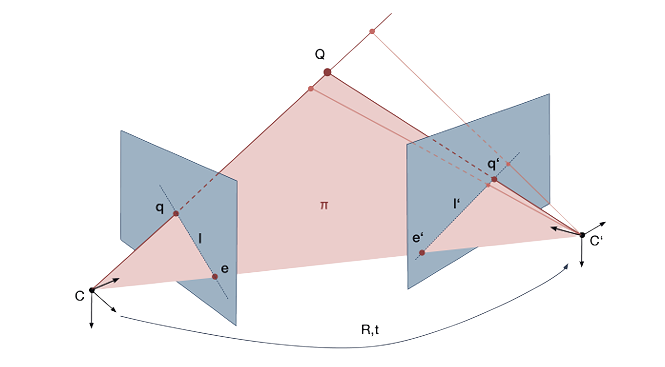
\includegraphics[width=0.8\textwidth]{images/epipolar_geometry.png}
\end{center}

\section*{Epipolar Geometry - Essential matrix}

\begin{equation*}
    E = [T_{\times} | R]
\end{equation*}

Where $T_x$ is the skew symmetric matrix associated to the translation vector and $R$ is the rotation matrix between the two camera image planes. \\

The skew symmetric matrix associated to a vector $a$ is defined as follows:

\begin{equation*}
    \begin{bmatrix}
        0 & -a_z & -a_y \\
        -a_z & 0 & -a_x \\
        -a_y & -a_x & 0
    \end{bmatrix}
\end{equation*}

It helps describing dot products as matrix multiplications:

\begin{equation*}
    a \times b = 
    \begin{bmatrix}
        0 & -a_z & -a_y \\
        -a_z & 0 & -a_x \\
        -a_y & -a_x & 0
    \end{bmatrix}
    \begin{bmatrix}
        b_x \\
        b_y \\
        b_z 
    \end{bmatrix} 
    = [a_{\times}] b
\end{equation*}

The \textbf{Essential matrix} is useful for computing the epipolar lines associated with $p$ and $p'$; for instance, given $p$ in the image plane of the first camera, $l' = E^Tp$ gives the epipolar line $l'$ in the image plane of the second camera. Similarly, $l = Ep'$ gives the epipolar line associated to $p'$ in the first image plane. An interesting property of the Essential matrix is that its dot product with the epipoles is $0$: $E^T e = E e' = 0$.\\

\textbf{We now have a way to map points and epipolar lines across views.} This only works for canonical cameras.

\newpage

\section*{Epipolar Geometry - Fundamental matrix}

\newpage 

\section*{Structure from motion}

We want to cover the three dimensional structure of an object; we start a video and move the camera around the subject. From the video we can abstract the object structure as well as the movement of the camera through space. How can we formulate the problem? What are the parameters we are trying to recover?\\

The structure from motion algorithm can be organized as a single matrix called \textbf{observation matrix}. We can basically rearrange the features tracked from the video into a single matrix containing the coordinates of the features. This matrix will have a very low rank (the maximal number of linearly independent columns) and this will allow us to use some constraint to decompose the observation matrix into two matrices: \textbf{structure matrix + motion matrix}. 

\begin{enumerate}
    \item Apply \textbf{feature detection to the first frame} of the video; the resulting features can be corners, SIFT features or any kind of interesting points. 
    \item \textbf{Track feature points}: this can be done with template matching, optical flow, by comparing SIFT descriptors etc. We end up getting \textbf{a set of tracked features};
\end{enumerate}

The image coordinates of this set of tracked features is the input for the structure from motion algorithm. \\

We have a world coordinate frame. Within this coordinate frame we have a set of N scene points of interest $p$.

\begin{equation*}
    p = 1, 2, ..., N\ points
\end{equation*}

We are taking images of this 3-dimensional structure. Each image give us a projection of these 3D points onto the 2D image. We have a sequence of such frames $f$. \\

\textbf{The structure from motion problem can be stated as:
Given sets of corresponding image points (2D): $(u_{f,p}, v_{f,p})$, find the scene points (3D) $P_p$, assuming an orthographic camera}. This means that the variation of depth that you have in the scene are assumed to be small compared to the distance of the scene from the camera; in other words the magnification of the camera remains constant for all points in the scene and through the entire sequence of images. 

\newpage

\section*{Structure from motion - math}

We can write the expression for the image of a point $P_p$ in camera frame $f$ as:

\begin{equation*}
    u_{f,p} = i_f^T(P_p-C_f)
\end{equation*}
\begin{equation*}
    v_{f,p} = j_f^T(P_p-C_f)
\end{equation*}

With $i, j$ being the orientation of the camera frame and $C_f$ being its center. Whats known for us is $(u_{f,p}, v_{f,p})$. We can remove one of the unknowns, $C_f$, using the \textbf{centering trick}: assume that the origin of the world coordinate frame lies on the centroid of the scene point we are trying to extract:

\begin{equation*}
    \frac{1}{N} \sum_{p=1}^N P_p = \dot p = 0
\end{equation*}

This means that when we recover the 3D coordinates of all of the scene points it will be with respect to this centroid. \\ 

Coordinates of the centroid in the camera frame $f$:
\begin{equation*}
    \dot u_f = \frac{1}{N} \sum_{p=1}^N u_{f, p} = \frac{1}{N} \sum_{p=1}^N i_f^T(P_p - C_f) = \frac{1}{N} i_f^T \sum_{p=1}^N P_p - \frac{1}{N} \sum_{p=1}^N i_f^T C_f
\end{equation*}

We said that $\frac{1}{N} i_f^T \sum_{p=1}^N P_p$, the sum of all the scene points, is $=0$ because we set the origin of our world coordinate frame at the centroid.

The sum $\frac{1}{N} \sum_{p=1}^N i_f^T C_f$ is a constant because neither $i_f^T$ and $C_f$ depend on $p$. We get:

\begin{equation*}
    \dot u_f = -i_f^T C_f
\end{equation*}

Same thing for $\dot v_f$:

\begin{equation*}
    \dot v_f = -j_f^T C_f
\end{equation*}

We can shift the camera origin to the centroid $(\dot u_f, \dot v_f)$ and define all the image coordinates in the new coordinate frame:

\begin{equation*}
    \dot u_{f, p} = u_{f,p} - \dot u_f = i_f^T (P_p - C_f) - i_f^T C_f = i_f^T C_f
\end{equation*}

\begin{equation*}
    \dot v_{f, p} = v_{f,p} - \dot v_f = j_f^T (P_p - C_f) - j_f^T C_f = j_f^T C_f
\end{equation*}

\textbf{Now we have the image coordinates of scene points but we no longer have the camera center in the expression.}  

The image coordinates can be written in vector form:

\begin{equation*}
    \begin{matrix}
        \dot u_{f, p} \\
        \dot v_{f, p}
    \end{matrix}
    = 
    \begin{bmatrix}
        i_f^T \\
        j_f^T
    \end{bmatrix}
    P_p 
\end{equation*}

This is valid for one point. We have $N$ points for $f$ frames. We will organize all these points into the \textbf{observation matrix}. Each row in the first half will contain all the $\dot u$ values for a single frame ($N$ values). We will have $f$ such rows. The second half will contain the $\dot v$ values in a similar fashion.

\begin{equation*}
    \begin{bmatrix}
        \dot u_{1,1} & \dot u_{1,2} & ... & \dot u_{1,N} \\
        \dot u_{2,1} & \dot u_{2,2} & ... & \dot u_{2,N} \\
        ... & ... & ... & ... \\
        \dot u_{F,1} & \dot u_{F,2} & ... & \dot u_{F,N} \\
        \dot v_{1,1} & \dot v_{1,2} & ... & \dot v_{1,N} \\
        \dot v_{2,1} & \dot v_{2,2} & ... & \dot v_{2,N} \\
        ... & ... & ... & ... \\
        \dot v_{F,1} & \dot v_{F,2} & ... & \dot v_{F,N}
    \end{bmatrix}
    =
    \begin{bmatrix}
        i_1^T \\
        i_2^T \\
        ... \\
        i_F^T \\
        j_1^T \\
        j_2^T \\
        ... \\
        j_F^T
    \end{bmatrix}
    \begin{bmatrix}
        P_1 & P_2 & ... & P_N
    \end{bmatrix}
\end{equation*}

\begin{equation*}
    \begin{matrix}
        W_{2F\times N} & \ \ & M_{2F_3} & S_{3\times N} \\
        \text{Observation matrix} & \ \ & \text{Camera Motion} & \text{Scene Structure} \\
        \text{(Centroid subtracted} & \ \ & \ \ & \ \ \\
        \text{Feature Points)} & \ \ & \ \ & \ \ \\
        \ \ & \ \ & \ \ & \ \ \\
        Known & \ \ & Unknown & Unknown
    \end{matrix}
\end{equation*}

The observation matrix will have a very low rank. The rank is the number of linear independent row vectors/column vectors of a matrix. Geometrically, the meaning of the rank is the dimensionality of the space spanned by the row/column vectors. The following property holds:

\begin{equation*}
    Rank(A) \leq min(m, n)
\end{equation*}

with $m, n$ being the dimensions of the matrix $A$. If you take the product of two matrices:

\begin{equation*}
    Rank(A_{m\times n}B_{n\times p}) = min(Rank(A_{m\times n}), Rank(B_{n\times p})) \leq min(m, n, p)
\end{equation*}

In our case:

\begin{equation*}
    \begin{matrix}
        Rank(MS) \leq Rank(M) & \ \ & Rank(MS) \leq Rank(S) \\
        Rank(MS) \leq min(3, 2F) & \ \ & Rank(MS) \leq min(3, N)
    \end{matrix}
\end{equation*}

Thus:
\begin{equation*}
    Rank(W) = Rank(MS) \leq min(3, N, 2F) = 3
\end{equation*}

\begin{equation*}
    Rank(W) \leq 3
\end{equation*}

\textbf{Now we have all it takes to develop the structure from motion algorithm.}

To factorize the observation matrix $W$ into $M$ and $S$ we will use a very popular technique called \textbf{singular value decomposition (SVD)} that can be applied to any matrix:

\begin{equation*}
    A_{m\times n} = U_{m\times m} \Sigma_{m\times n} V^T_{n\times n}
\end{equation*}

Where $U$ and $V$ are orthonormal matrices.
$\Sigma$ is a particularly important diagonal matrix:

\begin{equation*}
    \Sigma_{m\times n} = 
    \begin{bmatrix}
        \sigma_1 & 0 & ... & 0 \\
        0 & \sigma_2 & ... & 0 \\
        0 & 0 & ... & \sigma_N \\
        0 & 0 & ... & 0 \\
        ... & ... & ... & ...
    \end{bmatrix}
\end{equation*}

Where $\sigma_1 \geq \sigma_2 \geq ... \geq \sigma_N$ are the singular values of $W$. For a matrix $A$ with $m$ rows and $n$ columns, the singular values are defined as the square roots of the eigenvalues of the matrix $A^T A$ or $AA^T$. The singular values are $\sigma_1, \sigma_2, ..., \sigma_r$ , where $r$ is the rank of the matrix and $\sigma_1 \geq \sigma_2 \geq ... \geq \sigma_n \geq 0$. \\

Therefore, $W$ can have at most three non zero singular values. \textbf{We will have a massive matrix but just a few values will be $!= 0$.}

\begin{equation*}
    W = U \Sigma V =
\end{equation*}
\begin{equation*}
    \begin{bmatrix}
        U_1 & U_2\\
        (2F\times 3) & (2F\times 2F -3)
    \end{bmatrix}
    \begin{bmatrix}
        \sigma_1 & 0 & 0 & 0 & ... & 0 \\
        0 & \sigma_2 & 0 & 0 & ... & 0 \\
        0 & 0 & \sigma_3 & 0 & ... & 0 \\
        0 & 0 & 0 & 0 & ... & 0 \\
        ... & ... & ... & ... & ... & ...
    \end{bmatrix}
    \begin{bmatrix}
        V_1^T & (3\times N)\\
        V_2^T & (N-3\times N)
    \end{bmatrix}
\end{equation*}

\newpage

\section*{Structure from motion - steps}

\begin{itemize}
    \item Take a lot of images of an object;
    \item Identify points in the images that can possibly be detected in other images;
    \item Search for corresponding points in other images;
    \item Compute camera positions such that corresponding viewing rays intersect;
\end{itemize}


\end{comment}

\end{document}
